%%%%%%%%%%%%%%%%%%%%%%%%%%%%%%%%%%%%%%%%%
% Journal Article
% LaTeX Template
% Version 1.4 (15/5/16)
%
% This template has been downloaded from:
% http://www.LaTeXTemplates.com
%
% Original author:
% Frits Wenneker (http://www.howtotex.com) with extensive modifications by
% Vel (vel@LaTeXTemplates.com)
%
% License:
% CC BY-NC-SA 3.0 (http://creativecommons.org/licenses/by-nc-sa/3.0/)
%
%%%%%%%%%%%%%%%%%%%%%%%%%%%%%%%%%%%%%%%%%

%----------------------------------------------------------------------------------------
%	PACKAGES AND OTHER DOCUMENT CONFIGURATIONS
%----------------------------------------------------------------------------------------

\documentclass[twoside,twocolumn]{article}

\usepackage{blindtext} % Package to generate dummy text throughout this template 

\usepackage{hyperref}
\hypersetup{
    colorlinks=true,
    linkcolor=blue,
    filecolor=magenta,      
    urlcolor=cyan,
}

\usepackage[sc]{mathpazo} % Use the Palatino font
\usepackage[T1]{fontenc} % Use 8-bit encoding that has 256 glyphs
\linespread{1.05} % Line spacing - Palatino needs more space between lines
\usepackage{microtype} % Slightly tweak font spacing for aesthetics
\usepackage[utf8]{inputenc}

\usepackage[portuguese]{babel} % Language hyphenation and typographical rules

\usepackage[hmarginratio=1:1,top=32mm,columnsep=20pt]{geometry} % Document margins
\usepackage[hang, small,labelfont=bf,up,textfont=it,up]{caption} % Custom captions under/above floats in tables or figures
\usepackage{booktabs} % Horizontal rules in tables

\usepackage{lettrine} % The lettrine is the first enlarged letter at the beginning of the text
\usepackage{float}
\usepackage{enumitem} % Customized lists
\setlist[itemize]{noitemsep} % Make itemize lists more compact

\usepackage{abstract} % Allows abstract customization
\renewcommand{\abstractnamefont}{\normalfont\bfseries} % Set the "Abstract" text to bold
\renewcommand{\abstracttextfont}{\normalfont\small\itshape} % Set the abstract itself to small italic text
%\usepackage[shortlabels]{enumitem}
\usepackage{enumitem}
\usepackage{titlesec} % Allows customization of titles
\renewcommand\thesection{\Roman{section}} % Roman numerals for the sections
\renewcommand\thesubsection{\roman{subsection}} % roman numerals for subsections
\titleformat{\section}[block]{\large\scshape\centering}{\thesection.}{1em}{} % Change the look of the section titles
\titleformat{\subsection}[block]{\large}{\thesubsection.}{1em}{} % Change the look of the section titles

\usepackage{fancyhdr} % Headers and footers
\pagestyle{fancy} % All pages have headers and footers
\fancyhead{} % Blank out the default header
\fancyfoot{} % Blank out the default footer
\fancyhead[C]{MO443 $\bullet$ Maio 2019 $\bullet$ Relatório 03} % Custom header text
\fancyfoot[RO,LE]{\thepage} % Custom footer text

\usepackage{titling} % Customizing the title section

\usepackage{hyperref} % For hyperlinks in the PDF

\usepackage{graphicx}
\usepackage{subfigure}

\usepackage{mathtools}
\DeclarePairedDelimiter\floor{\lfloor}{\rfloor}
%----------------------------------------------------------------------------------------
%	TITLE SECTION
%----------------------------------------------------------------------------------------

\setlength{\droptitle}{-4\baselineskip} % Move the title up

\pretitle{\begin{center}\Huge\bfseries} % Article title formatting
\posttitle{\end{center}} % Article title closing formatting
\title{Relatório - Trabalho 03 \\ \Large MO443 - Introdução ao Processamento de Imagem Digital} %
%\subtitle{qsdqwdqwd} %Article title
\author{%
\textsc{Vinicius Teixeira de Melo - RA: 230223} \\[1ex] % Your name
\normalsize Universidade Estadual de Campinas \\ % Your institution
\normalsize \href{mailto:viniciusteixeira@liv.ic.unicamp.br}{viniciusteixeira@liv.ic.unicamp.br} % Your email address
%\and % Uncomment if 2 authors are required, duplicate these 4 lines if more
%\textsc{Jane Smith}\thanks{Corresponding author} \\[1ex] % Second author's name
%\normalsize University of Utah \\ % Second author's institution
%\normalsize \href{mailto:jane@smith.com}{jane@smith.com} % Second author's email address
}
\date{\today} % Leave empty to omit a date
\renewcommand{\maketitlehookd}{%
%\begin{abstract}
%\noindent \blindtext % Dummy abstract text - replace \blindtext with your abstract text
%\end{abstract}
}

%----------------------------------------------------------------------------------------

\begin{document}

% Print the title
\maketitle

%----------------------------------------------------------------------------------------
%	ARTICLE CONTENTS
%----------------------------------------------------------------------------------------

\section{Especificação do Problema}

O objetivo deste trabalho é aplicar operadores morfológicos para segmentar regiões compreendendo texto e
não texto em uma imagem de entrada.

Os seguintes passos devem ser realizados:

\begin{enumerate}
	\item dilatação da imagem original com um elemento estruturante de 1 pixel de altura e 100 pixels de largura;
	\item erosão da imagem resultante com o mesmo elemento estruturante do passo (1);
	\item dilatação da imagem original com um elemento estruturante de 200 pixels de altura e 1 pixel de largura;
	\item erosão da imagem resultante com o mesmo elemento estruturante do passo (3);
	\item aplicação da intersecção (AND) dos resultados dos passos (2) e (4);
	\item fechamento do resultado obtido no passo (5) com um elemento estruturante de 1 pixel de altura e 30
pixels de largura;
	\item aplicação de algoritmo para identificação de componentes conexos (ver programa fornecido) sobre o
resultado do passo (6);
	\item para cada retângulo envolvendo um objeto, calcule:
	\begin{enumerate}
		\item razão entre o número de pixels pretos e o número total de pixels (altura x largura);
		\item razão entre o número de transições verticais e horizontais branco para preto e o número total de pixels pretos;
	\end{enumerate}
	\item criação de uma regra para classificar cada componente conexo, de acordo com as medidas obtidas no
passo (8), como texto e não texto.
	\item aplicação de operadores morfológicos apropriados para segmentar cada linha do texto em blocos de palavras. Coloque um retângulo envolvendo cada palavra na imagem original. Calcule o número total de linhas de texto e de blocos de palavras na imagem.
\end{enumerate}

%------------------------------------------------

\section{Entrada de Dados}

O código fonte criado para a execução de todas as tarefas está no notebook \textbf{Trabalho 03.ipynb}. O código foi criado para aceitar imagens em preto e branco no formato PBM (\textit{Portable Bitmap}).

Para executar o notebook, basta iniciar o ambiente \textit{Jupyter Notebook}, abrir o notebook \textbf{Trabalho 03.ipynb} e executar as células em ordem. Todo o algoritmo foi implementado na linguagem Python na versão 3.6.

As imagen de entrada utilizada no teste do algoritmo foi retirada da página do prof. Hélio Pedrini: \href{http://www.ic.unicamp.br/~helio/imagens_morfologia/}{Imagens}. Na pasta \textbf{imgs/} está a imagem em preto e branco utilizada no teste: \textbf{bitmap.pbm}. As dimensões da imagen de entrada utilizada é 1374 x 2233.

\begin{figure}[H]
\begin{center}
	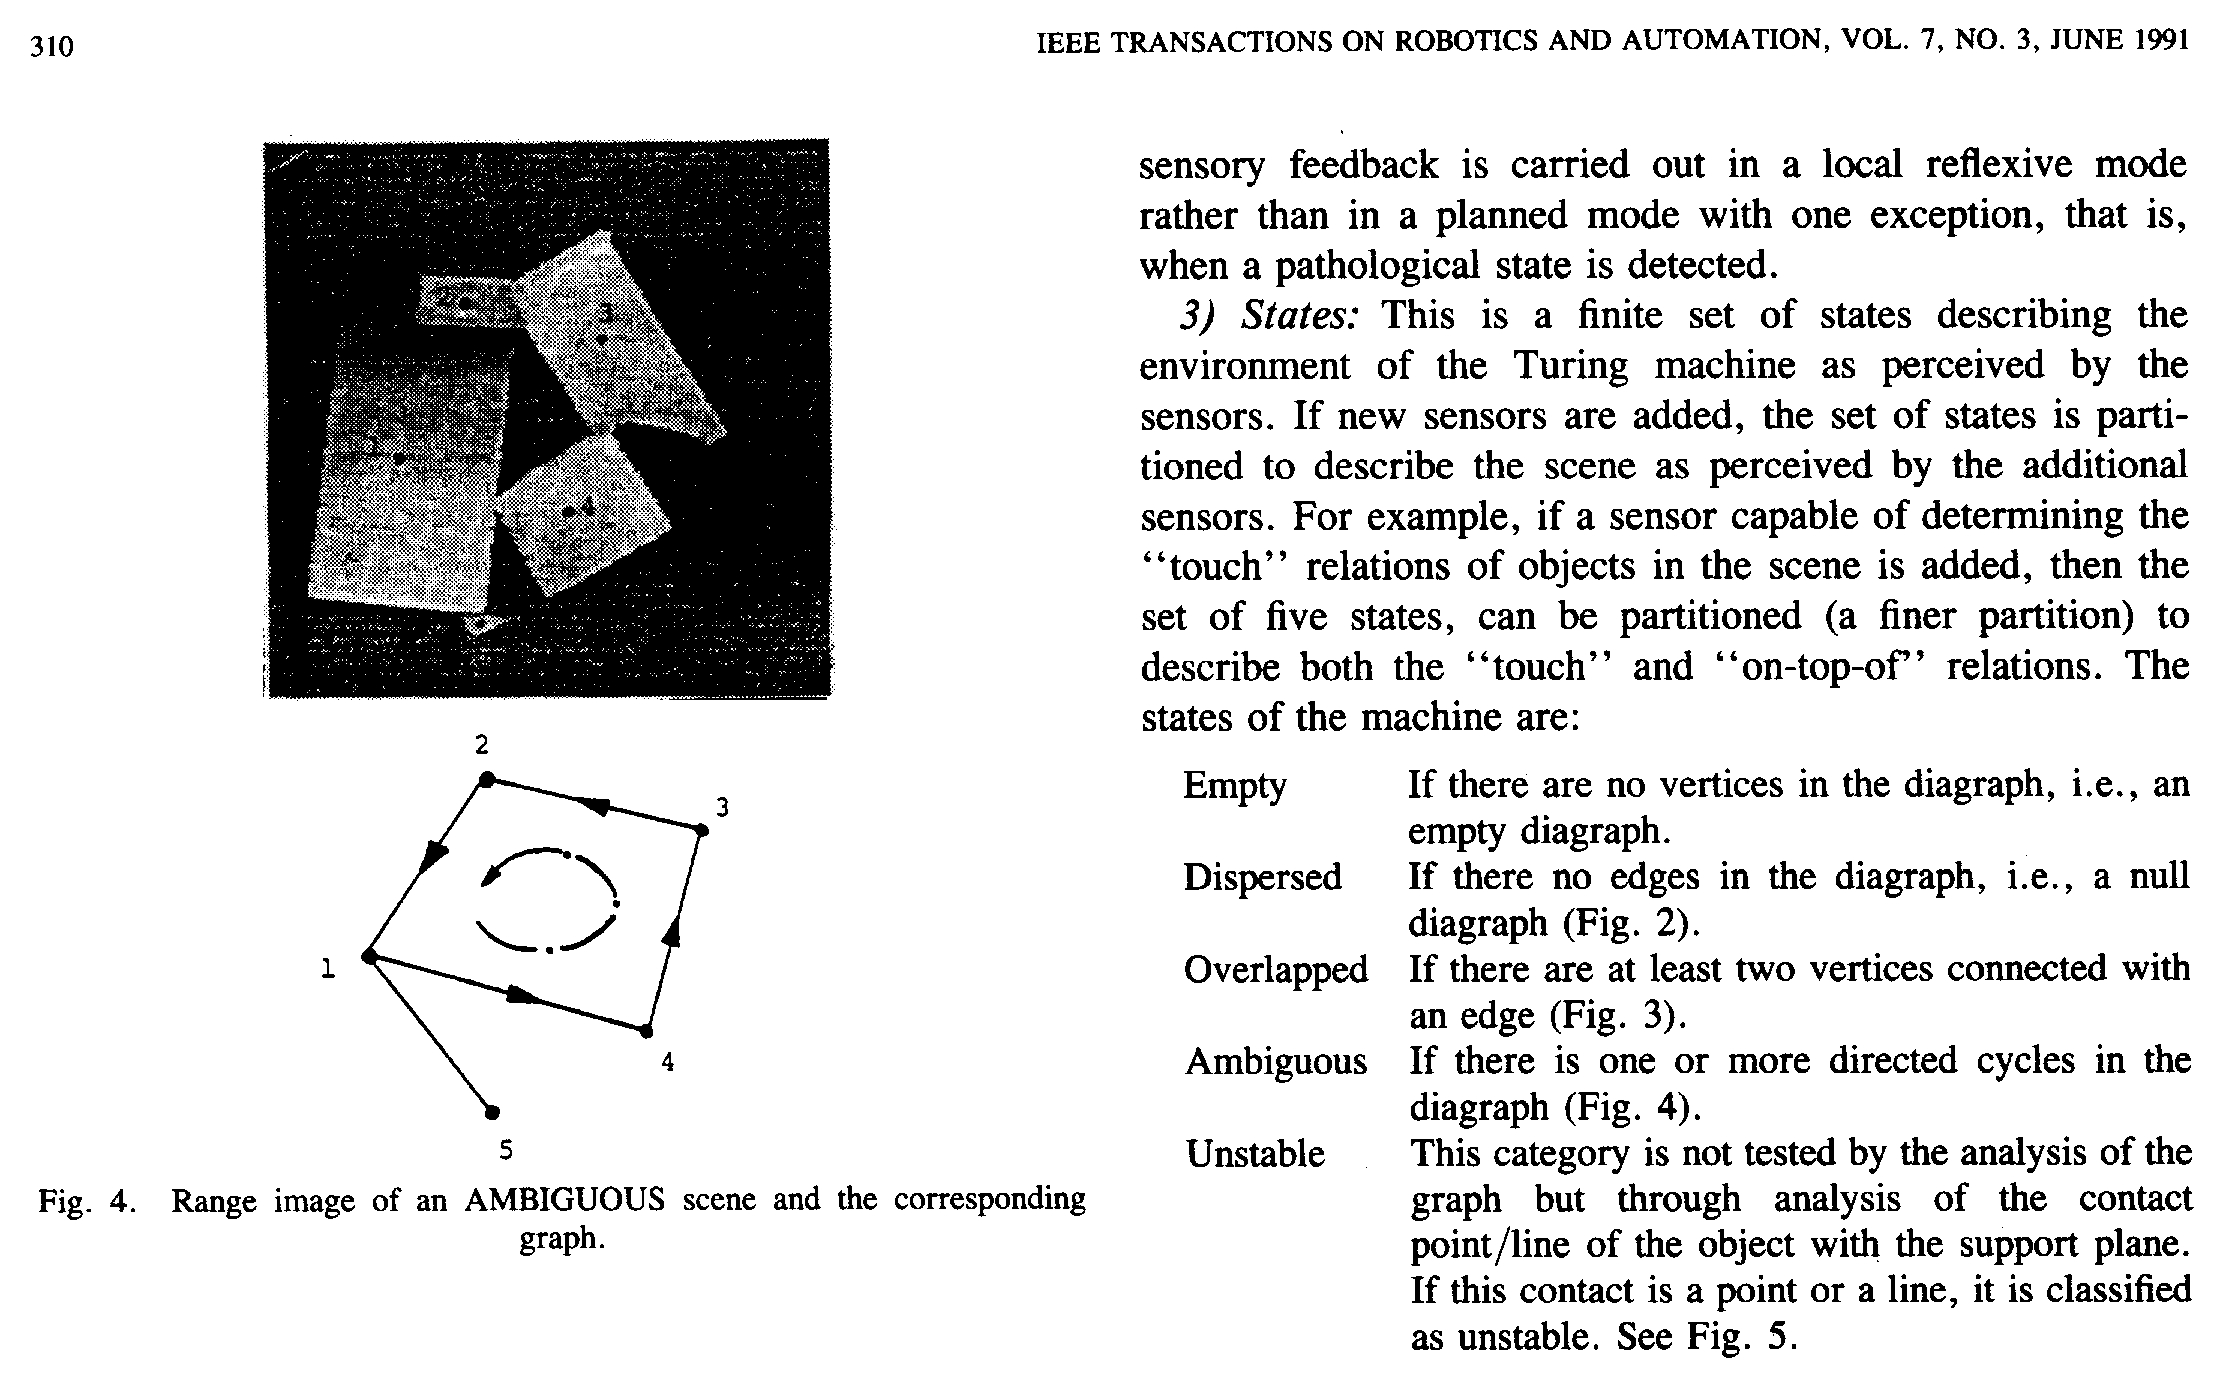
\includegraphics[height=4cm]{figures/bitmap.png}
\caption{bitmap.pbm} \label{gdimotes}
\end{center}
\end{figure}

%------------------------------------------------

\section{Dependências e Códigos}

As bibliotecas utilizadas neste trabalho foram:

\begin{table}[H]
\begin{tabular}{|l|l|}
\hline
\textbf{Biblioteca} & \textbf{Versão} \\ \hline
numpy               & 1.16.2          \\ \hline
cv2                 & 3.4.2           \\ \hline
matplotlib          & 3.0.3           \\ \hline
warnings            & 2.1             \\ \hline
\end{tabular}
\end{table}

A leitura das imagens foi realizada utilizando uma função do \textbf{opencv} \cite{b1} chamada \textbf{imread()}, a qual necessitou de uma constante do próprio \textbf{opencv} para que a imagem ficassem apenas com o canal de escala de cinza, essa constante é denominada \textbf{IMREAD\_GRAYSCALE}.

Os elementos estruturantes foram criados manualmente através da função \textbf{np.ones((\textit{shape}),np.uint8)}. Primeiramente, a imagem de entrada foi transformada para que as áreas de interesse estivessem com valor $255$. Para as operações de \textit{bits}, foram utilizadas as funções \textbf{cv2.bitwise\_not} e \textbf{cv2.bitwise\_and}.

Nas operações fundamentais de morfologia foram utilizadas com base nas funções \textbf{cv2.dilate} e \textbf{cv2.erose}. Para a operação de fechamento, foi utilizada a função \textbf{cv2.morphologyEx} com a constante do próprio OpenCv, chamada \textbf{cv2.MORPH\_CLOSE}.

No passo (7), para a detecção de componentes e criação dos \textit{bounding boxes} foi utilizada a função \textbf{cv2.findContours}, juntamente com as constantes \textbf{cv2.RETR\_TREE} e \textbf{cv2.CHAIN\_APPROX\_SIMPLE}. Assim, após a obtenção dos \textit{bounding boxes}, foram utilizadas as funções \textbf{cv2.boundingRect}, \textbf{cv2.rectangle} e \textbf{cv2.drawContours} para desenhar os \textit{bounding boxes} na imagem de entrada.

No passo (9), a regra utilizada para classificar um \textit{bounding box} como texto ou não foi: dado o valor $x_{a}$ obtido no passo (8.a) e o valor $x_{b}$ obtido no passo (8.b) referentes ao mesmo \textit{bounding box}, se $|x_{a} - x_{b}| \leq 0.2$, esse \textit{bounding box} é classificado como texto, se não, é classificado como não texto.


%------------------------------------------------

\section{Fundamentação}

\subsection{Morfologia Matemática}

A morfologia matemática se refere ao estudo e análise de imagens usando operadores não lineares. Dentre as atividades que a morfologia executa no processamento de imagens estão: aumento de qualidade, restauração, detecção de falhas, análise da textura, análise particular, análise de formas, compreensão, dentre outras. Essas ferramentas são aplicadas em diversas áreas como visão em robos, inspeções, microscopia, biologia, metalurgia e documentos digitais. Ambas áreas e técnicas continuam a se expandir.

O processo da morfologia se baseia na geometria, em um contexto bem específico. A idéia básica é percorrer uma imagem com um elemento estruturante e quantificar a maneira com que este se encaixa ou não na imagem. No caso afirmativo, marca-se o local ou nível de cinza onde o elemento estruturante coube na imagem. Dessa forma, pode-se extrair informações relevantes sobre o tamanho e forma de estruturas na imagem.

\subsubsection{Dilatação}

A operação de dilatação entre o conjunto $A$ e o elemento estruturante $B$ é definida como a \textit{adição de Minkowski}, ou seja

\begin{equation}
	\mathcal{D}(A,B) = A \oplus B = \bigcup_{b \in B} (A + b).
\end{equation}

O processo de dilatação entre $A$ e $B$ corresponde ao conjunto de todas as translações de $B$ com os pontos da imagem em que há pelo menos um elemento não nulo (pixel com valor 1) em comum com o conjunto A.

\subsubsection{Erosão}

A operação de erosão entre o conjunto $A$ e o elemento estruturante $B$ é definida como a subtração de \textit{Minkowski}, ou seja

\begin{equation}
	\mathcal{E}(A,B) = A \ominus B = \bigcap_{b \in B} (A - b).
\end{equation}

A erosão de $A$ por $B$ é o conjunto de todos os elementos de $B$ transladados por $p$ que estão contidas em $A$. Entretanto, deve-se observar que o resultado da erosão de uma imagem pode não ser um subconjunto de imagem original, caso o elemento estruturante não contenha a origem.

\subsubsection{Fechamento}

O fechamento de $A$ por $B$, denotado por $A \bullet B$, é definido como

\begin{equation}
	A \bullet B = (A \oplus B) \ominus B
\end{equation}

o qual pode ser interpretado geometricamente como a união de todas as translações de $B$ que não estão contidas em $A$.

%------------------------------------------------

\section{Saída de Dados}

As imagens resultantes foram salvas dentro da pasta \textbf{resultados/} utilizando uma função da biblioteca \textbf{opencv} chamada \textbf{cv2.imwrite()} \cite{b1}.

O formato dos nomes de saída estão da seguinte forma: para cada passo do problema, é salva uma imagem com o nome ''bitmap\_(passo)'', e no passo número 10 é uma imagem referente a todos os componentes conexos e outra somente com os componentes que foram classificados como palavras.

%------------------------------------------------

\section{Resultados e Discuções}

Os resultados obtidos com a aplicação do passo a passo definido no problema estão a seguir:

\begin{figure}[H]
\begin{center}
	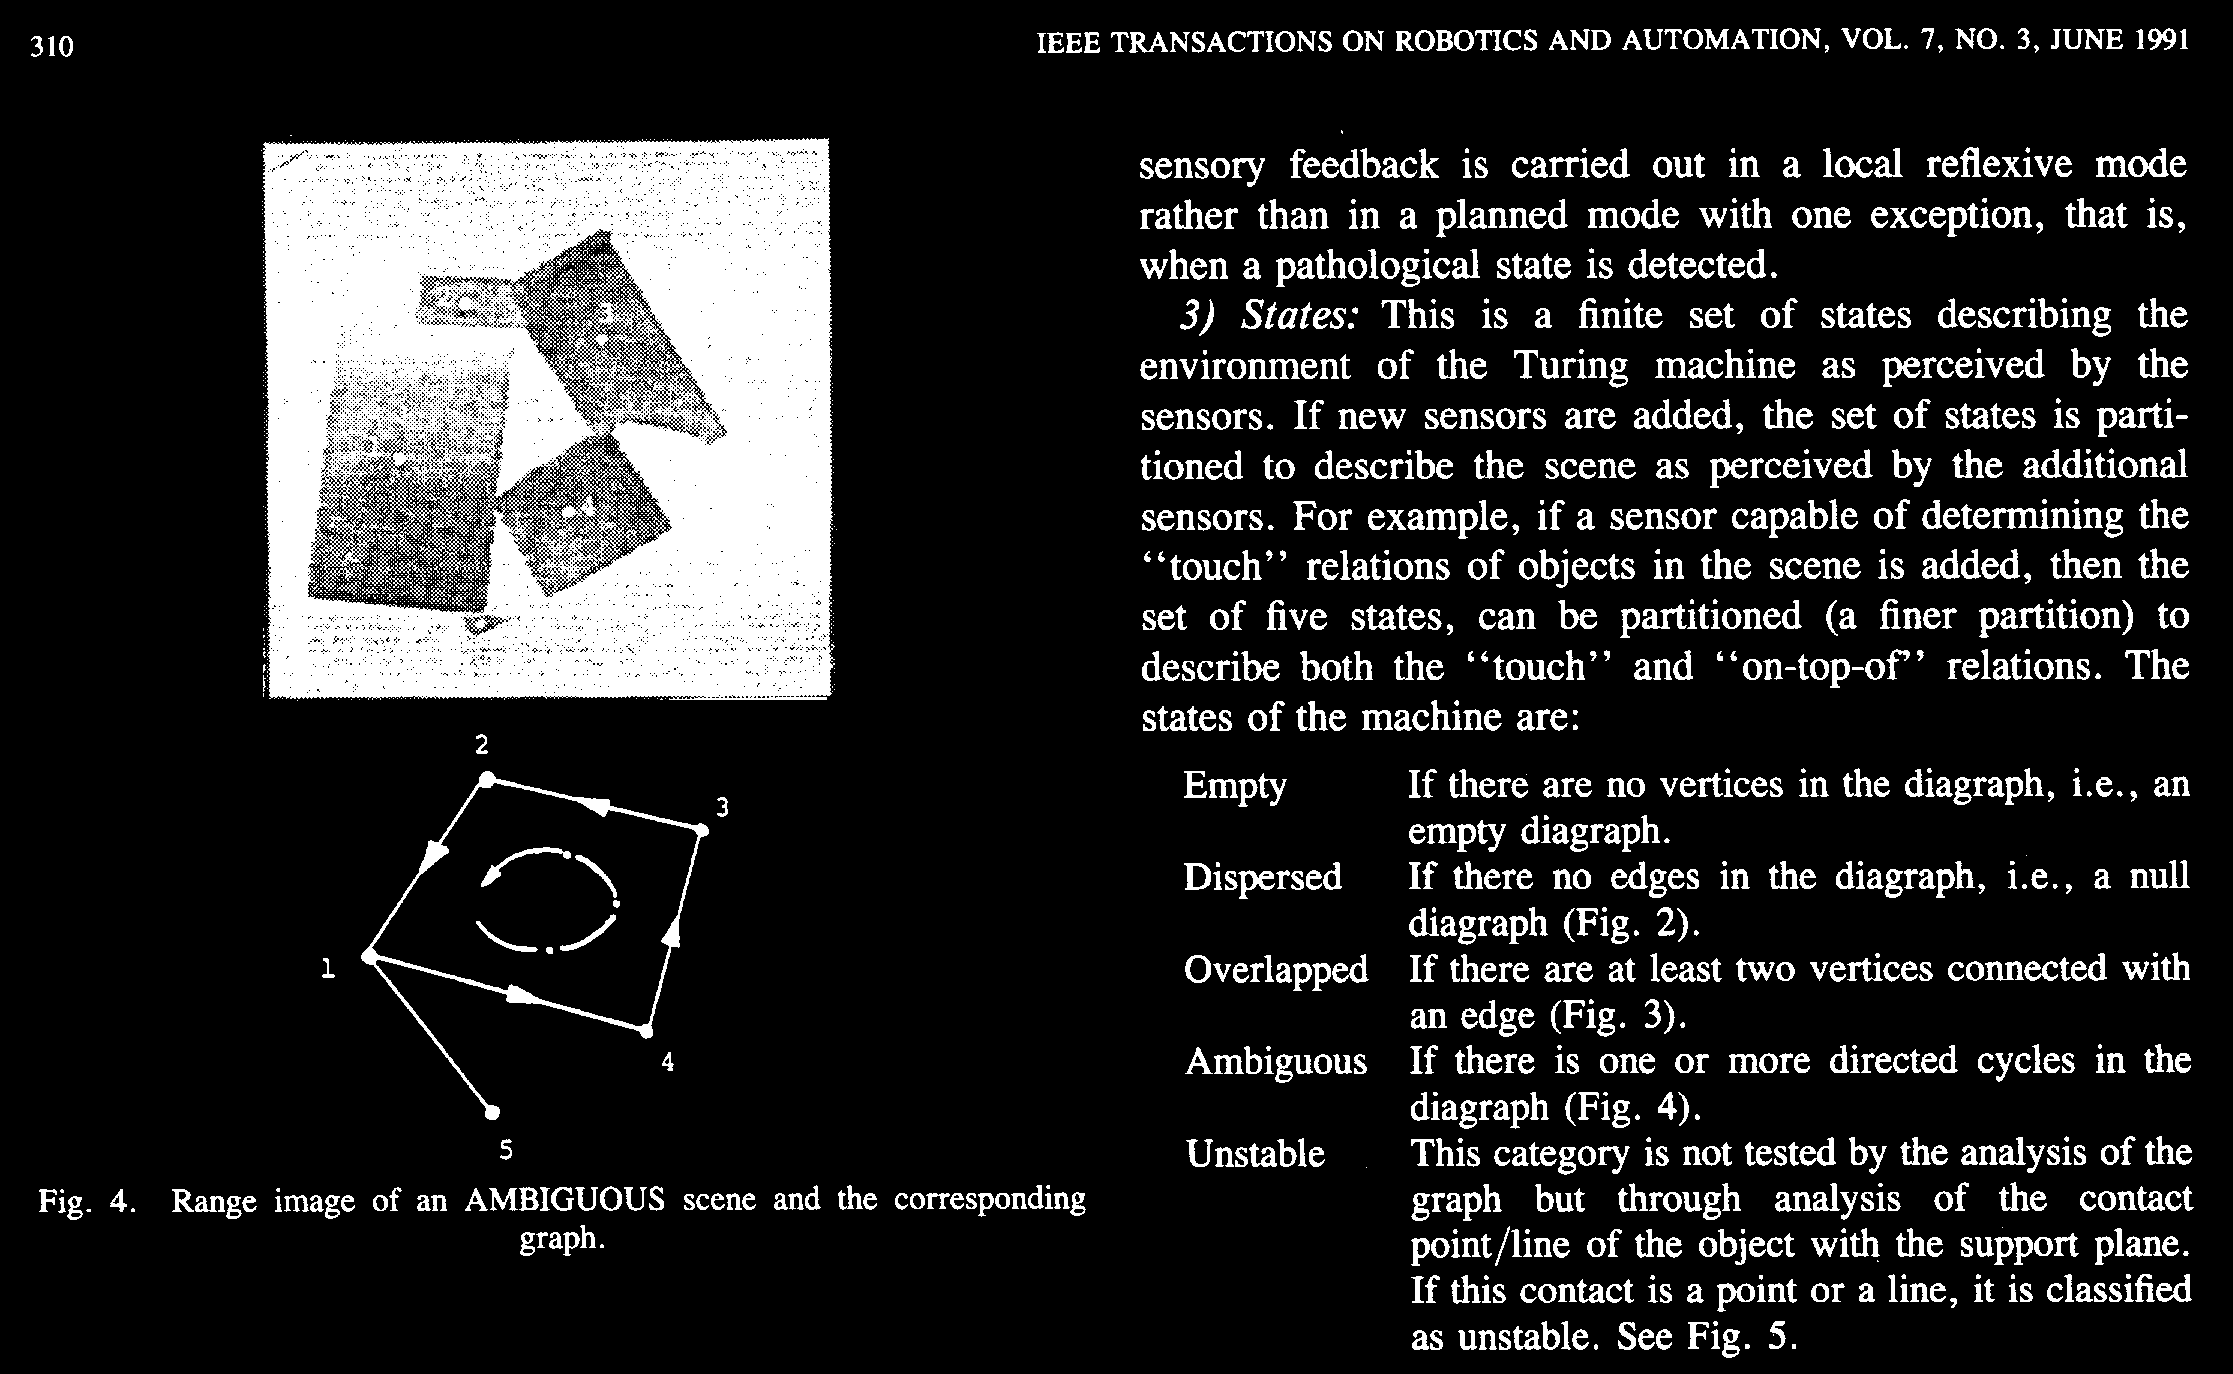
\includegraphics[height=4cm]{figures/bitmap_not.png}
\caption{bitmap\_not.pbm} \label{bitmap_not}
\end{center}
\end{figure}

Primeiramente, para a aplicação das operação básicas de morfologia matemática, a imagem de entrada foi transformada em ''negativa''. Os \textit{pixels} que tinham o valor $255$ passaram a ter valor $0$ e os \textit{pixels} que tinham valor $0$ passaram a ter o valor $255$. O resultado dessa operação é mostrado na Figura~\ref{bitmap_not}.

\begin{figure}[H]
\begin{center}
	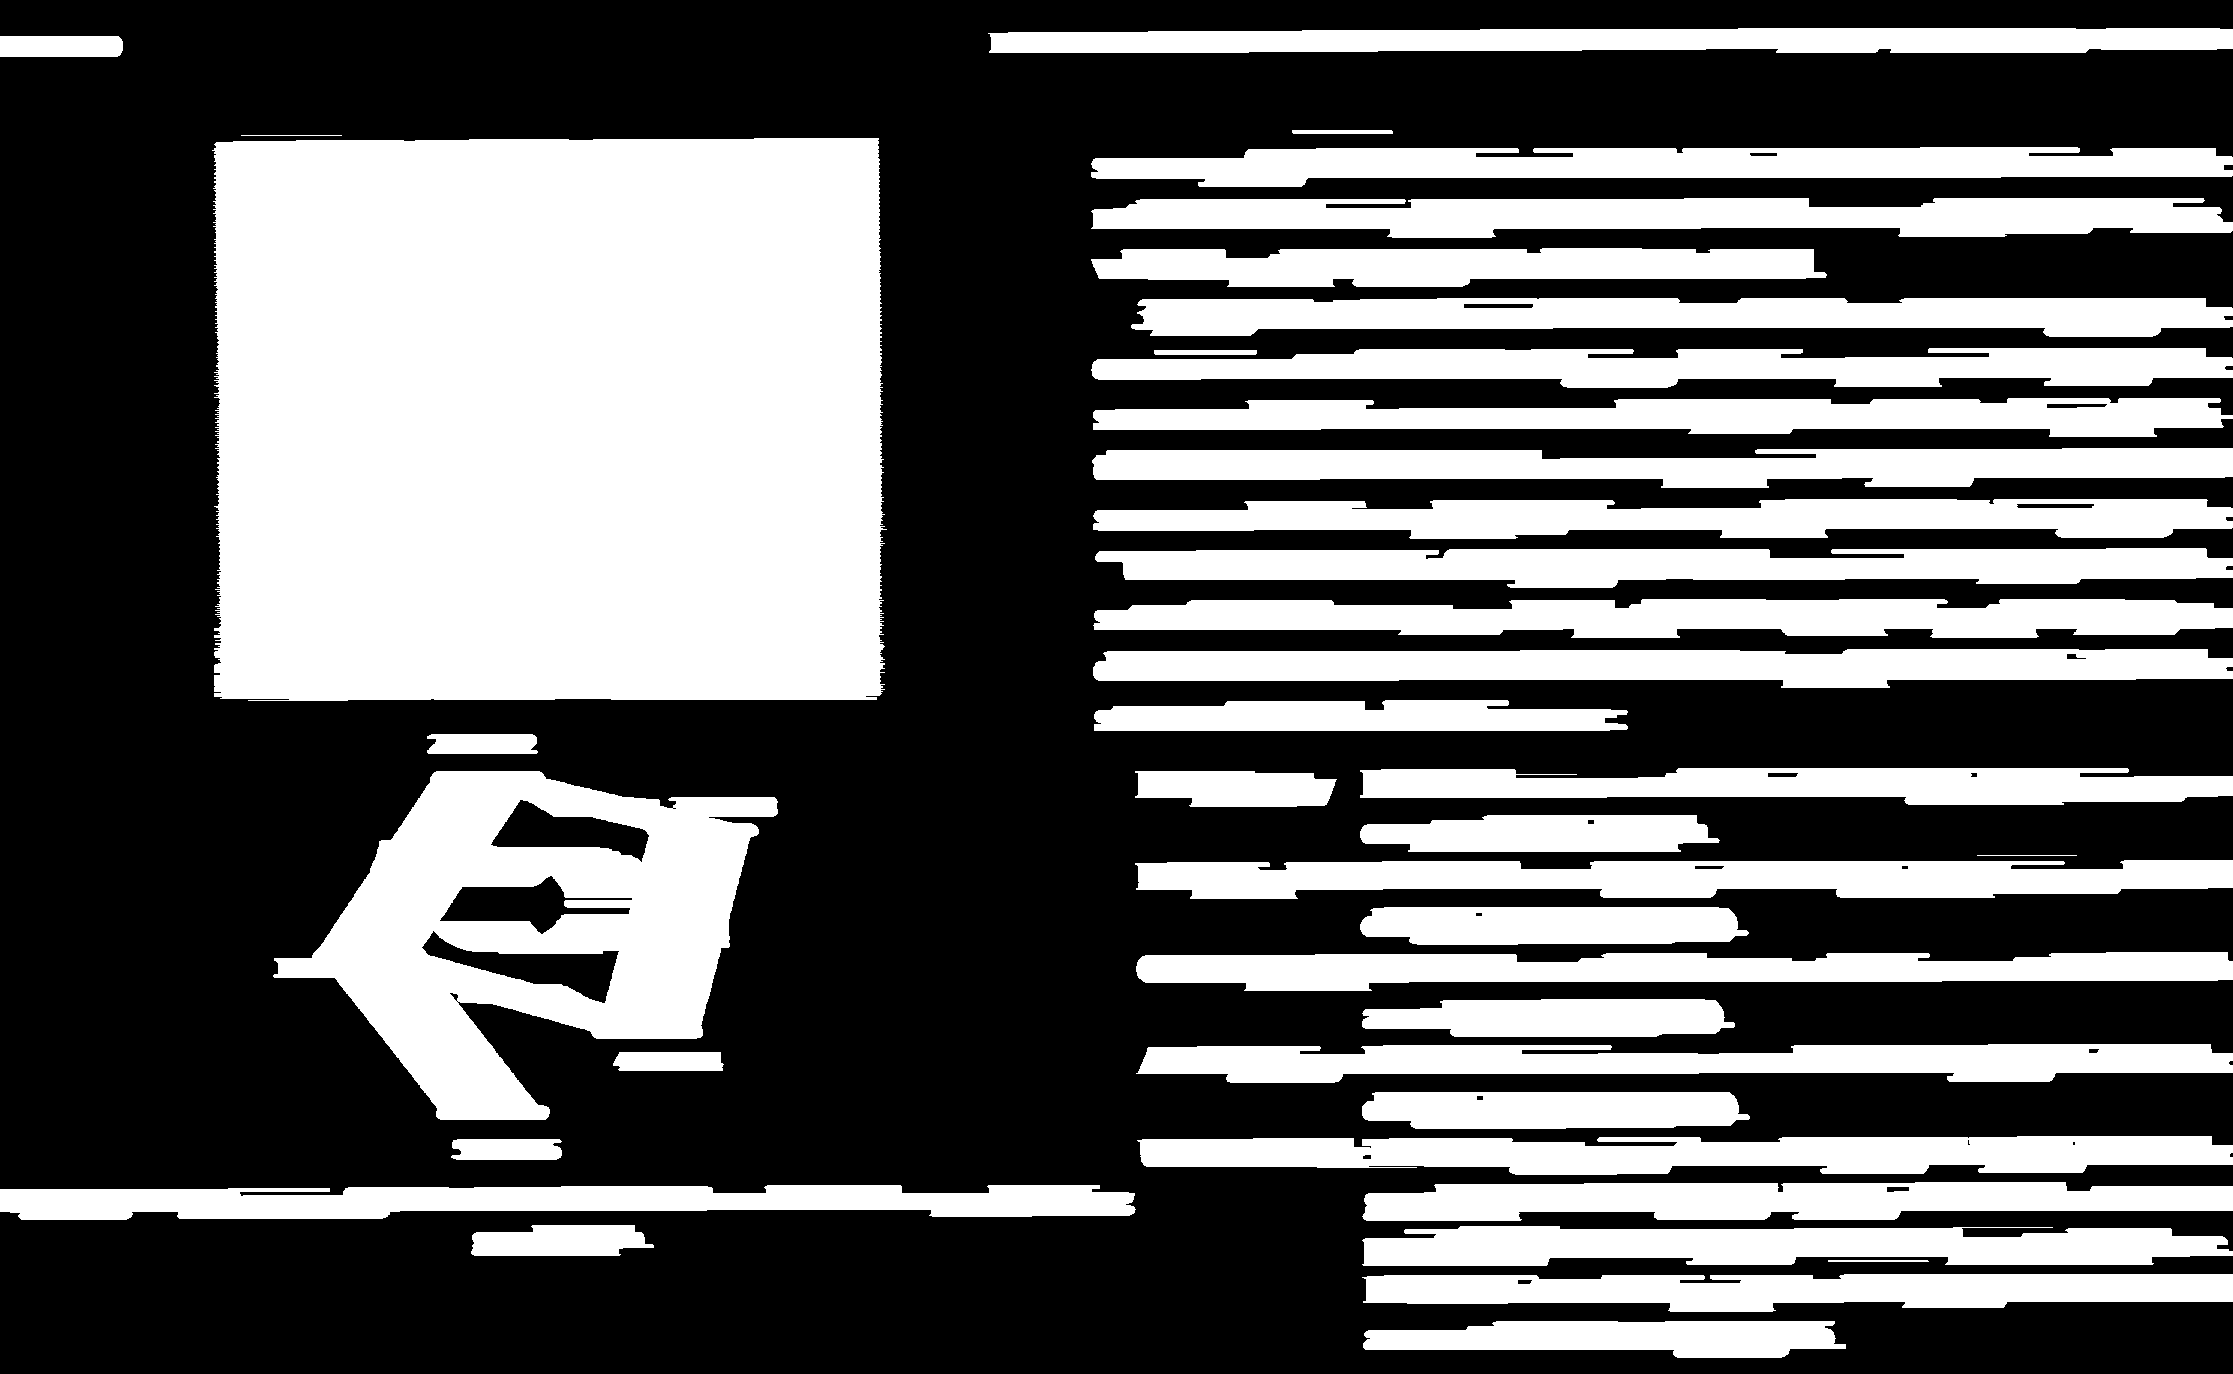
\includegraphics[height=4cm]{figures/step_1.png}
\caption{Passo (1)} \label{step_1}
\end{center}
\end{figure}

A Figura~\ref{step_1} apresenta o resultado da dilatação da imagem original com um elemento estruturante de 1 \textit{pixel} de altura e 100 \textit{pixels} de largura. Como resultado temos uma imagem em que os componentes foram alargados e alguns foram unidos, formando um componente conexo mais abrangente. Podemos observar os componentes que estavam separados em uma mesma linha agora estão formando somente um componente. E como o elemento estruturante é maior na horizontal, podemos observar que os componentes tiveram sua largura aumentada.

\begin{figure}[H]
\begin{center}
	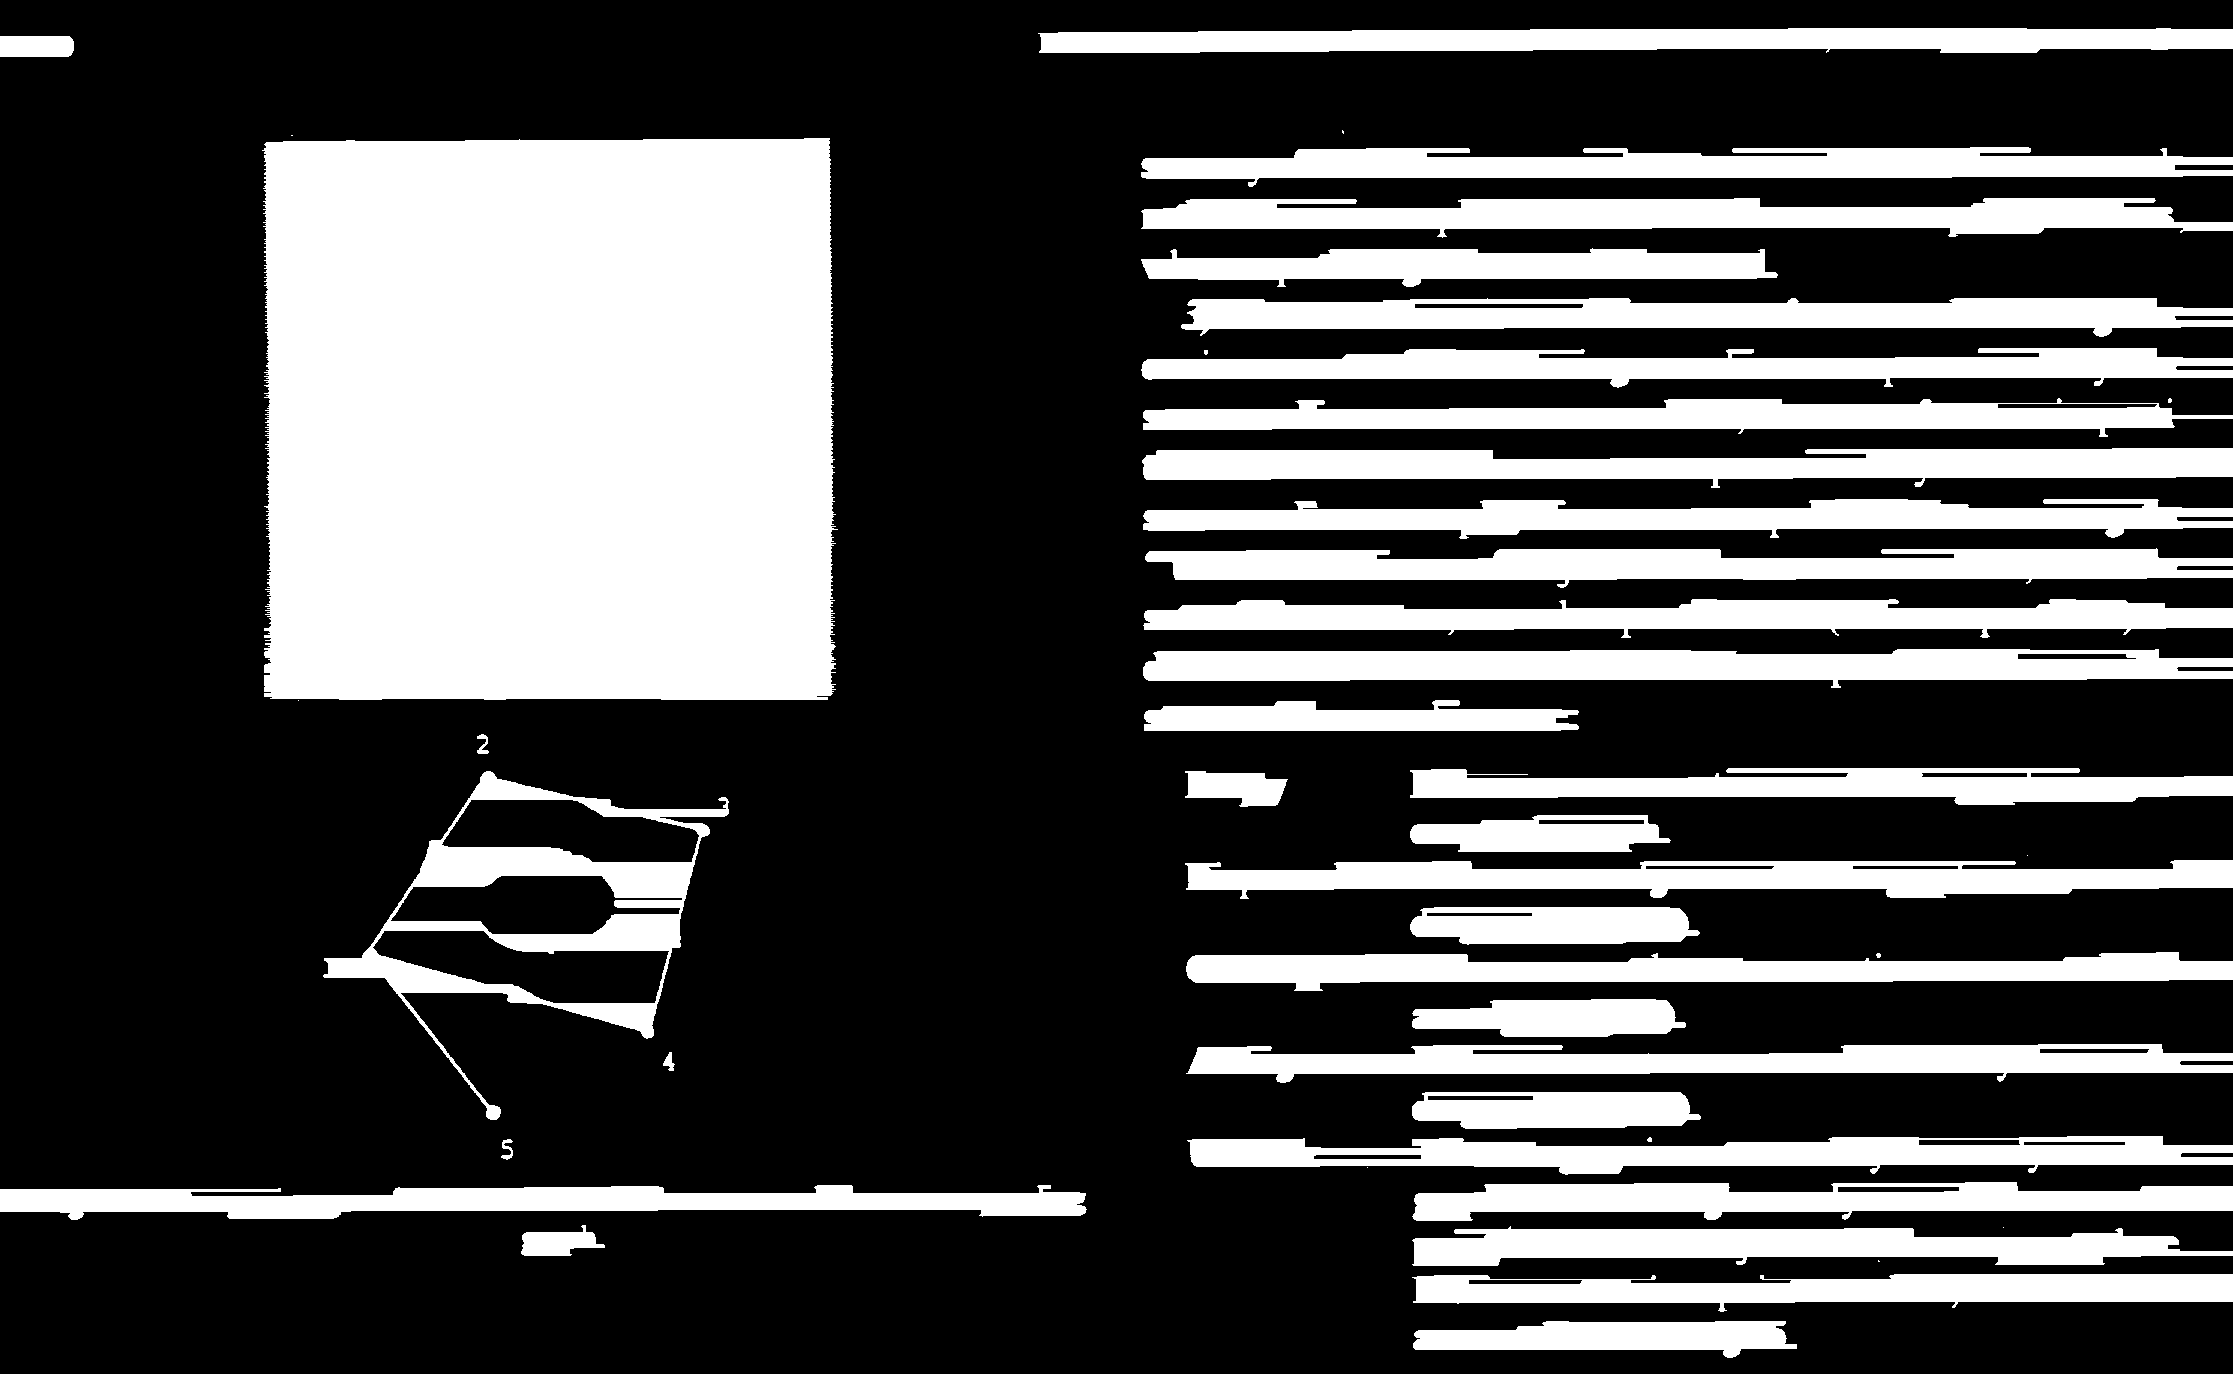
\includegraphics[height=4cm]{figures/step_2.png}
\caption{Passo (2)} \label{step_2}
\end{center}
\end{figure}

A Figura~\ref{step_2} apresenta o resultado da erosão da imagem da Figura~\ref{step_1} com o mesmo elemento estruturante do passo (1). Podemos observar que com essa operação de erosão a imagem sofreu um redução na parte externa das componentes conexas, assim é possível fazer uma analogia com um ''afinamento'' dessas componentes. Com esse passo, podemos ver também que o espaçamento entre as linhas ficou mais bem definido.

\begin{figure}[H]
\begin{center}
	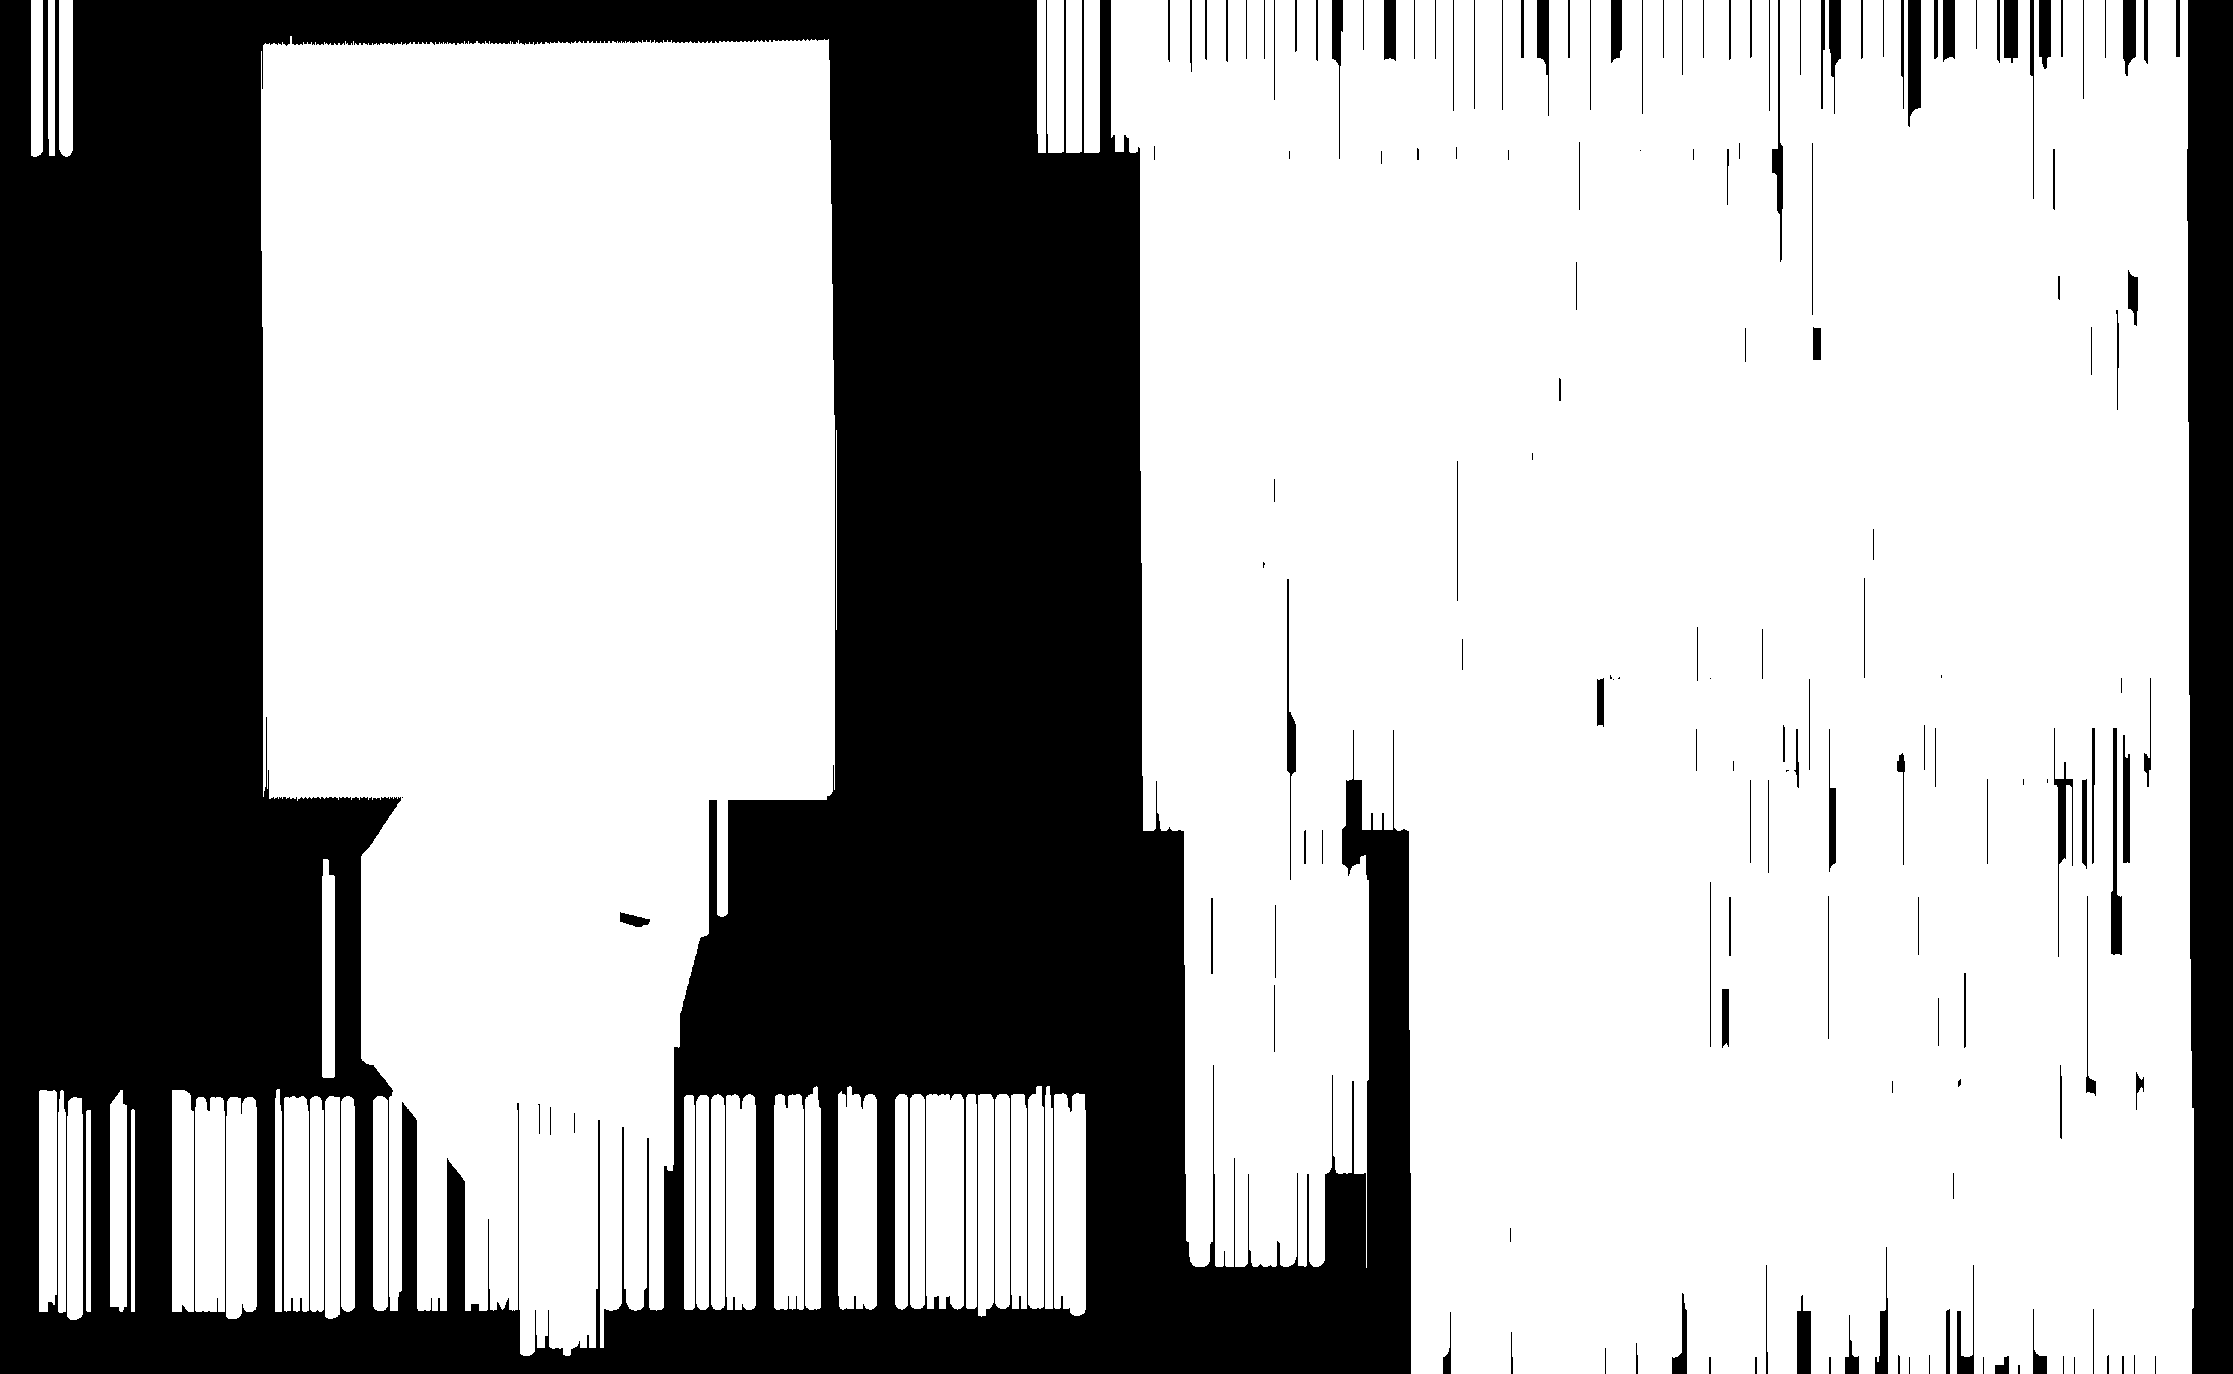
\includegraphics[height=4cm]{figures/step_3.png}
\caption{Passo (3)} \label{step_3}
\end{center}
\end{figure}

A Figura~\ref{step_3} apresenta o resultado da dilatação da imagem original com o elemento estruturante de 200 \textit{pixels} de altura e 1 \textit{pixel} de largura. Podemos observar que a imagem sofreu um alargamento das componentes na vertical, resultando assim na união de muitos componentes.

\begin{figure}[H]
\begin{center}
	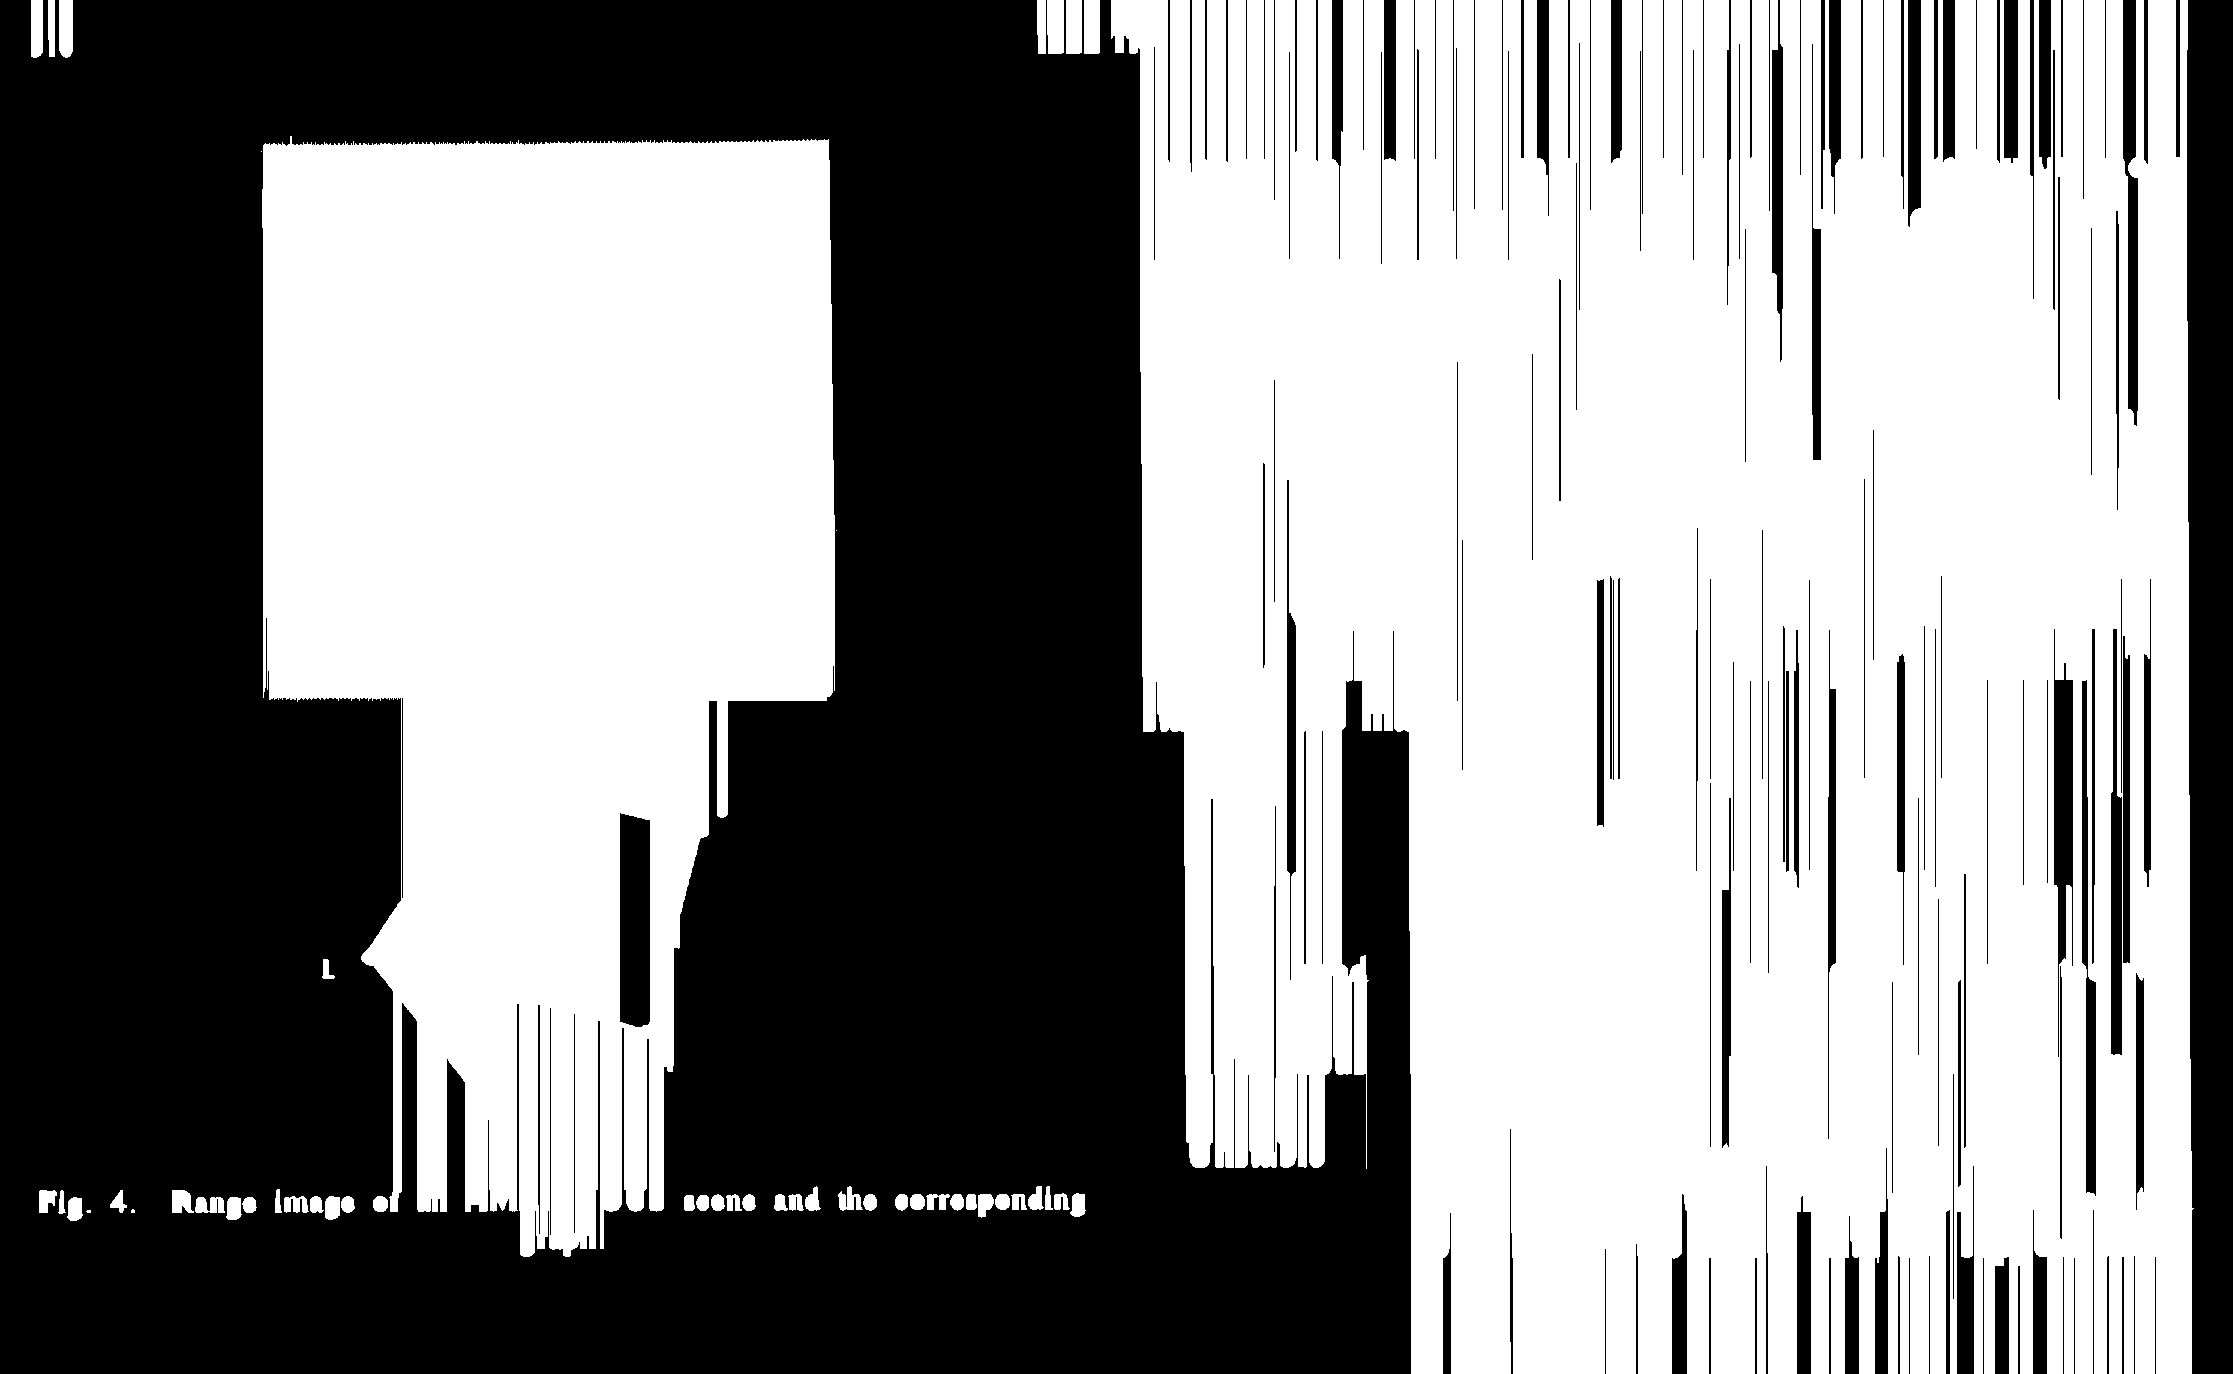
\includegraphics[height=4cm]{figures/step_4.png}
\caption{Passo (4)} \label{step_4}
\end{center}
\end{figure}

A Figura~\ref{step_4} apresenta o resultado da erosão da imagem da Figura~\ref{step_3} com o mesmo elemento do passo (3). Podemos observar que ocorreu a remoção de uma camada externa dos componentes conexos, e os componentes que não ocupavam uma área considerável foram ''excluídos''.

\begin{figure}[H]
\begin{center}
	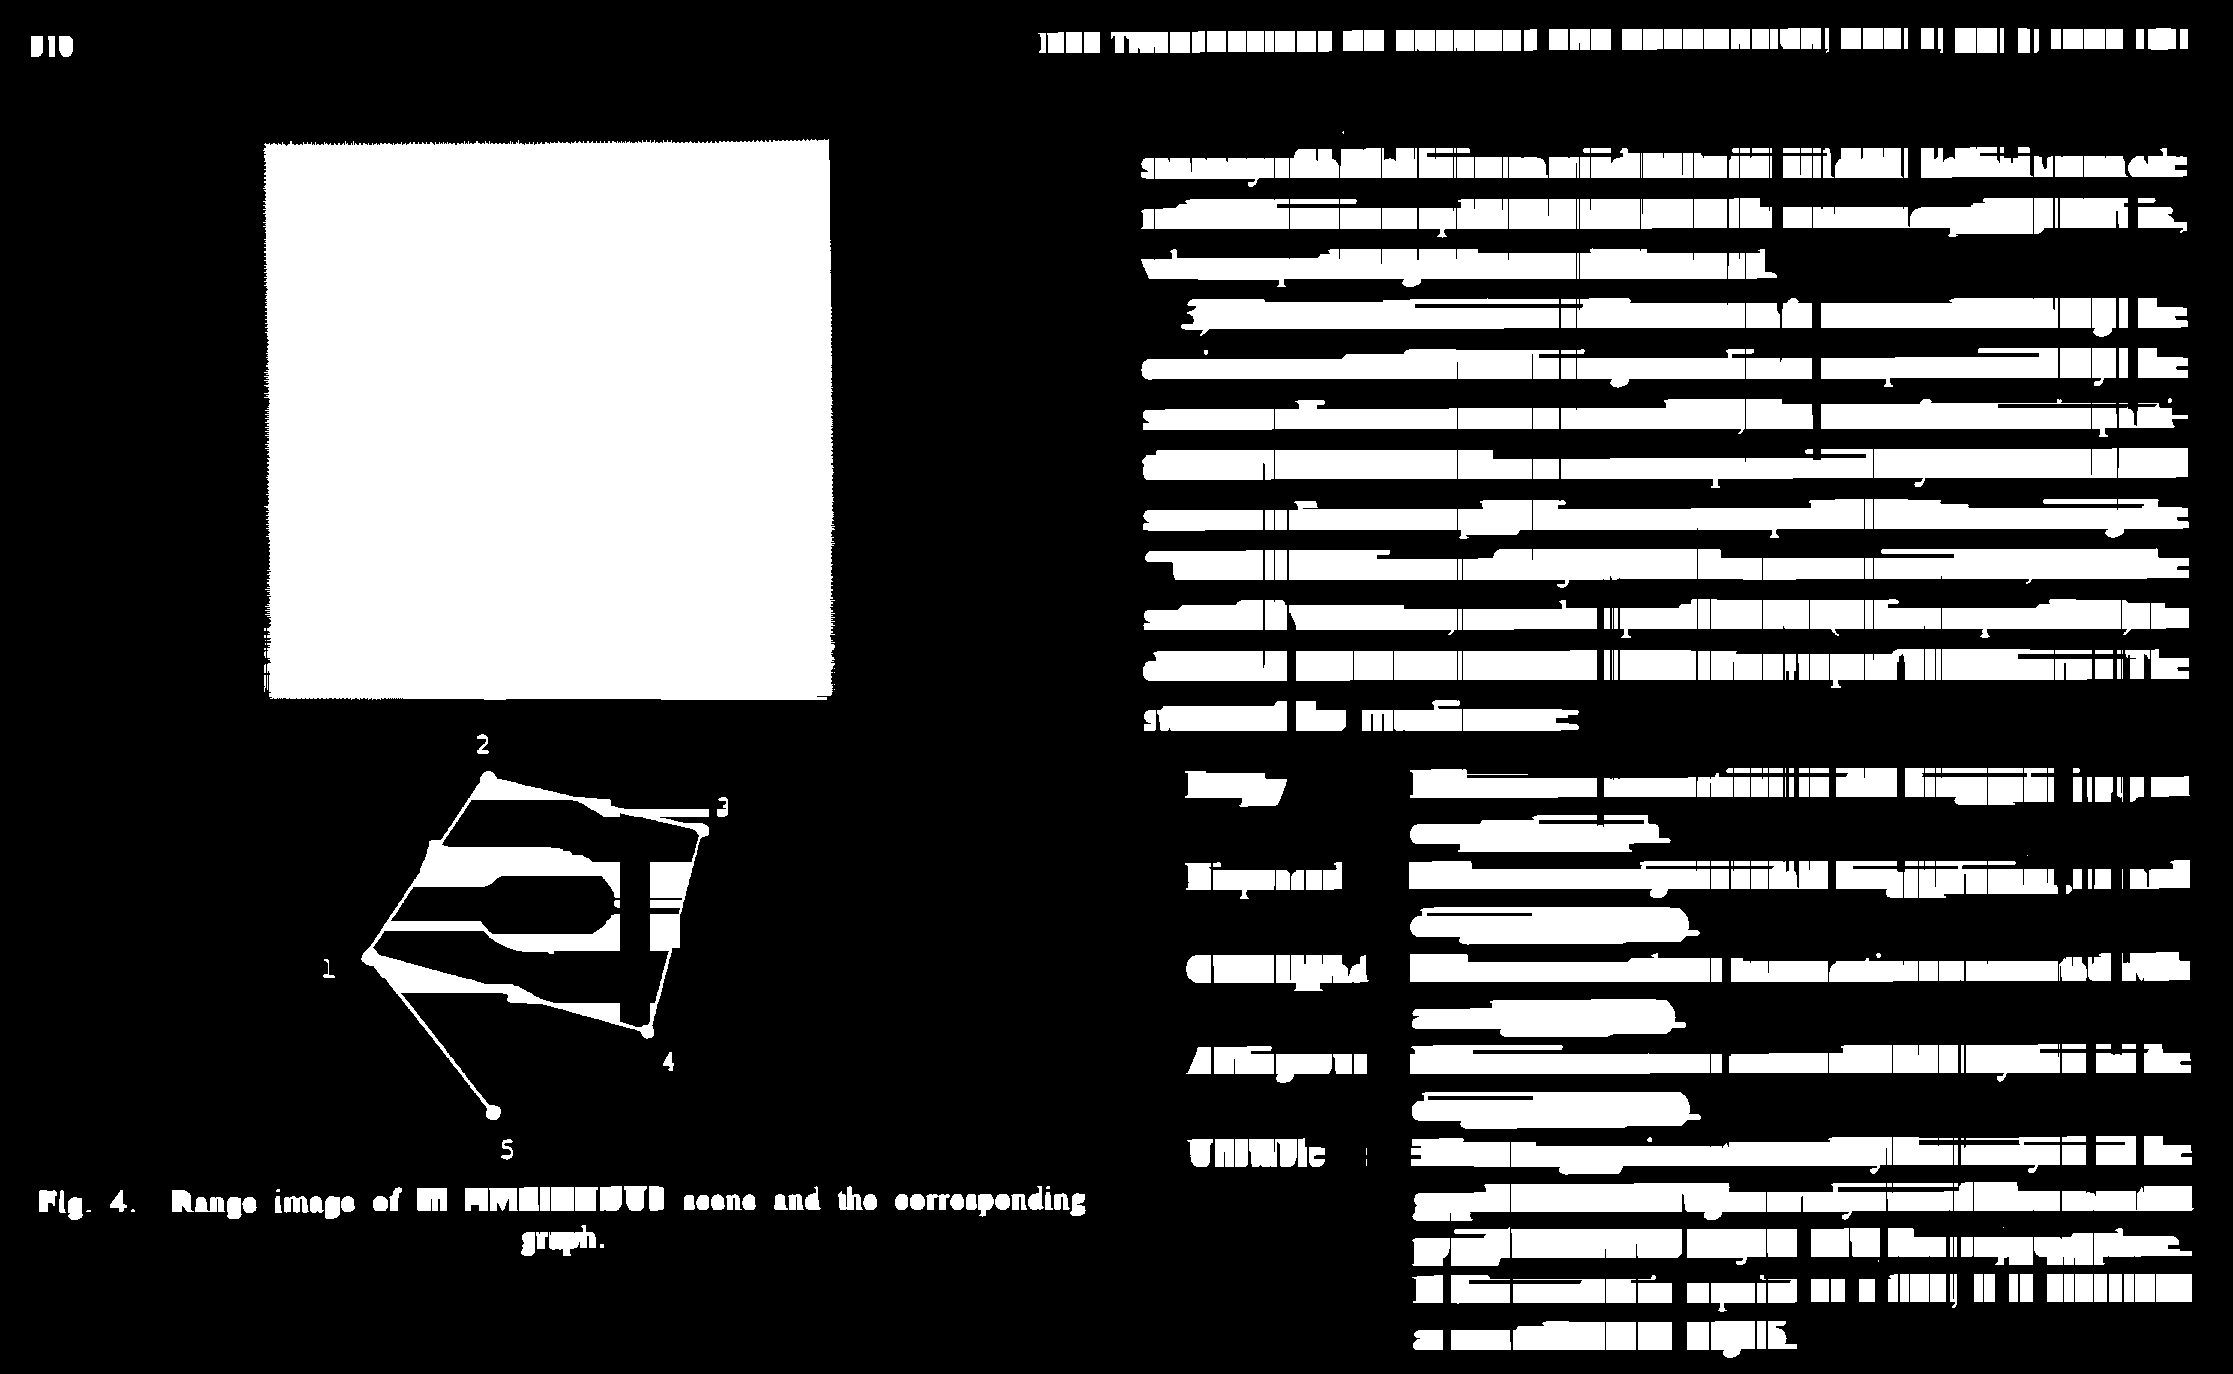
\includegraphics[height=4cm]{figures/step_5.png}
\caption{Passo (5)} \label{step_5}
\end{center}
\end{figure}

A Figura~\ref{step_5} apresenta o resultado da operação de \textit{AND} entre a imagem obtida após o passo (2) e o passo (4). Com essa operação, a imagem resultante mantém os \textit{pixels} que tinham o valor $255$ nas duas imagens, assim, a imagem resultante mantém a divisão por linhas e ainda separações entre componentes de uma mesma linha, obtidas através da imagem do passo (4).

\begin{figure}[H]
\begin{center}
	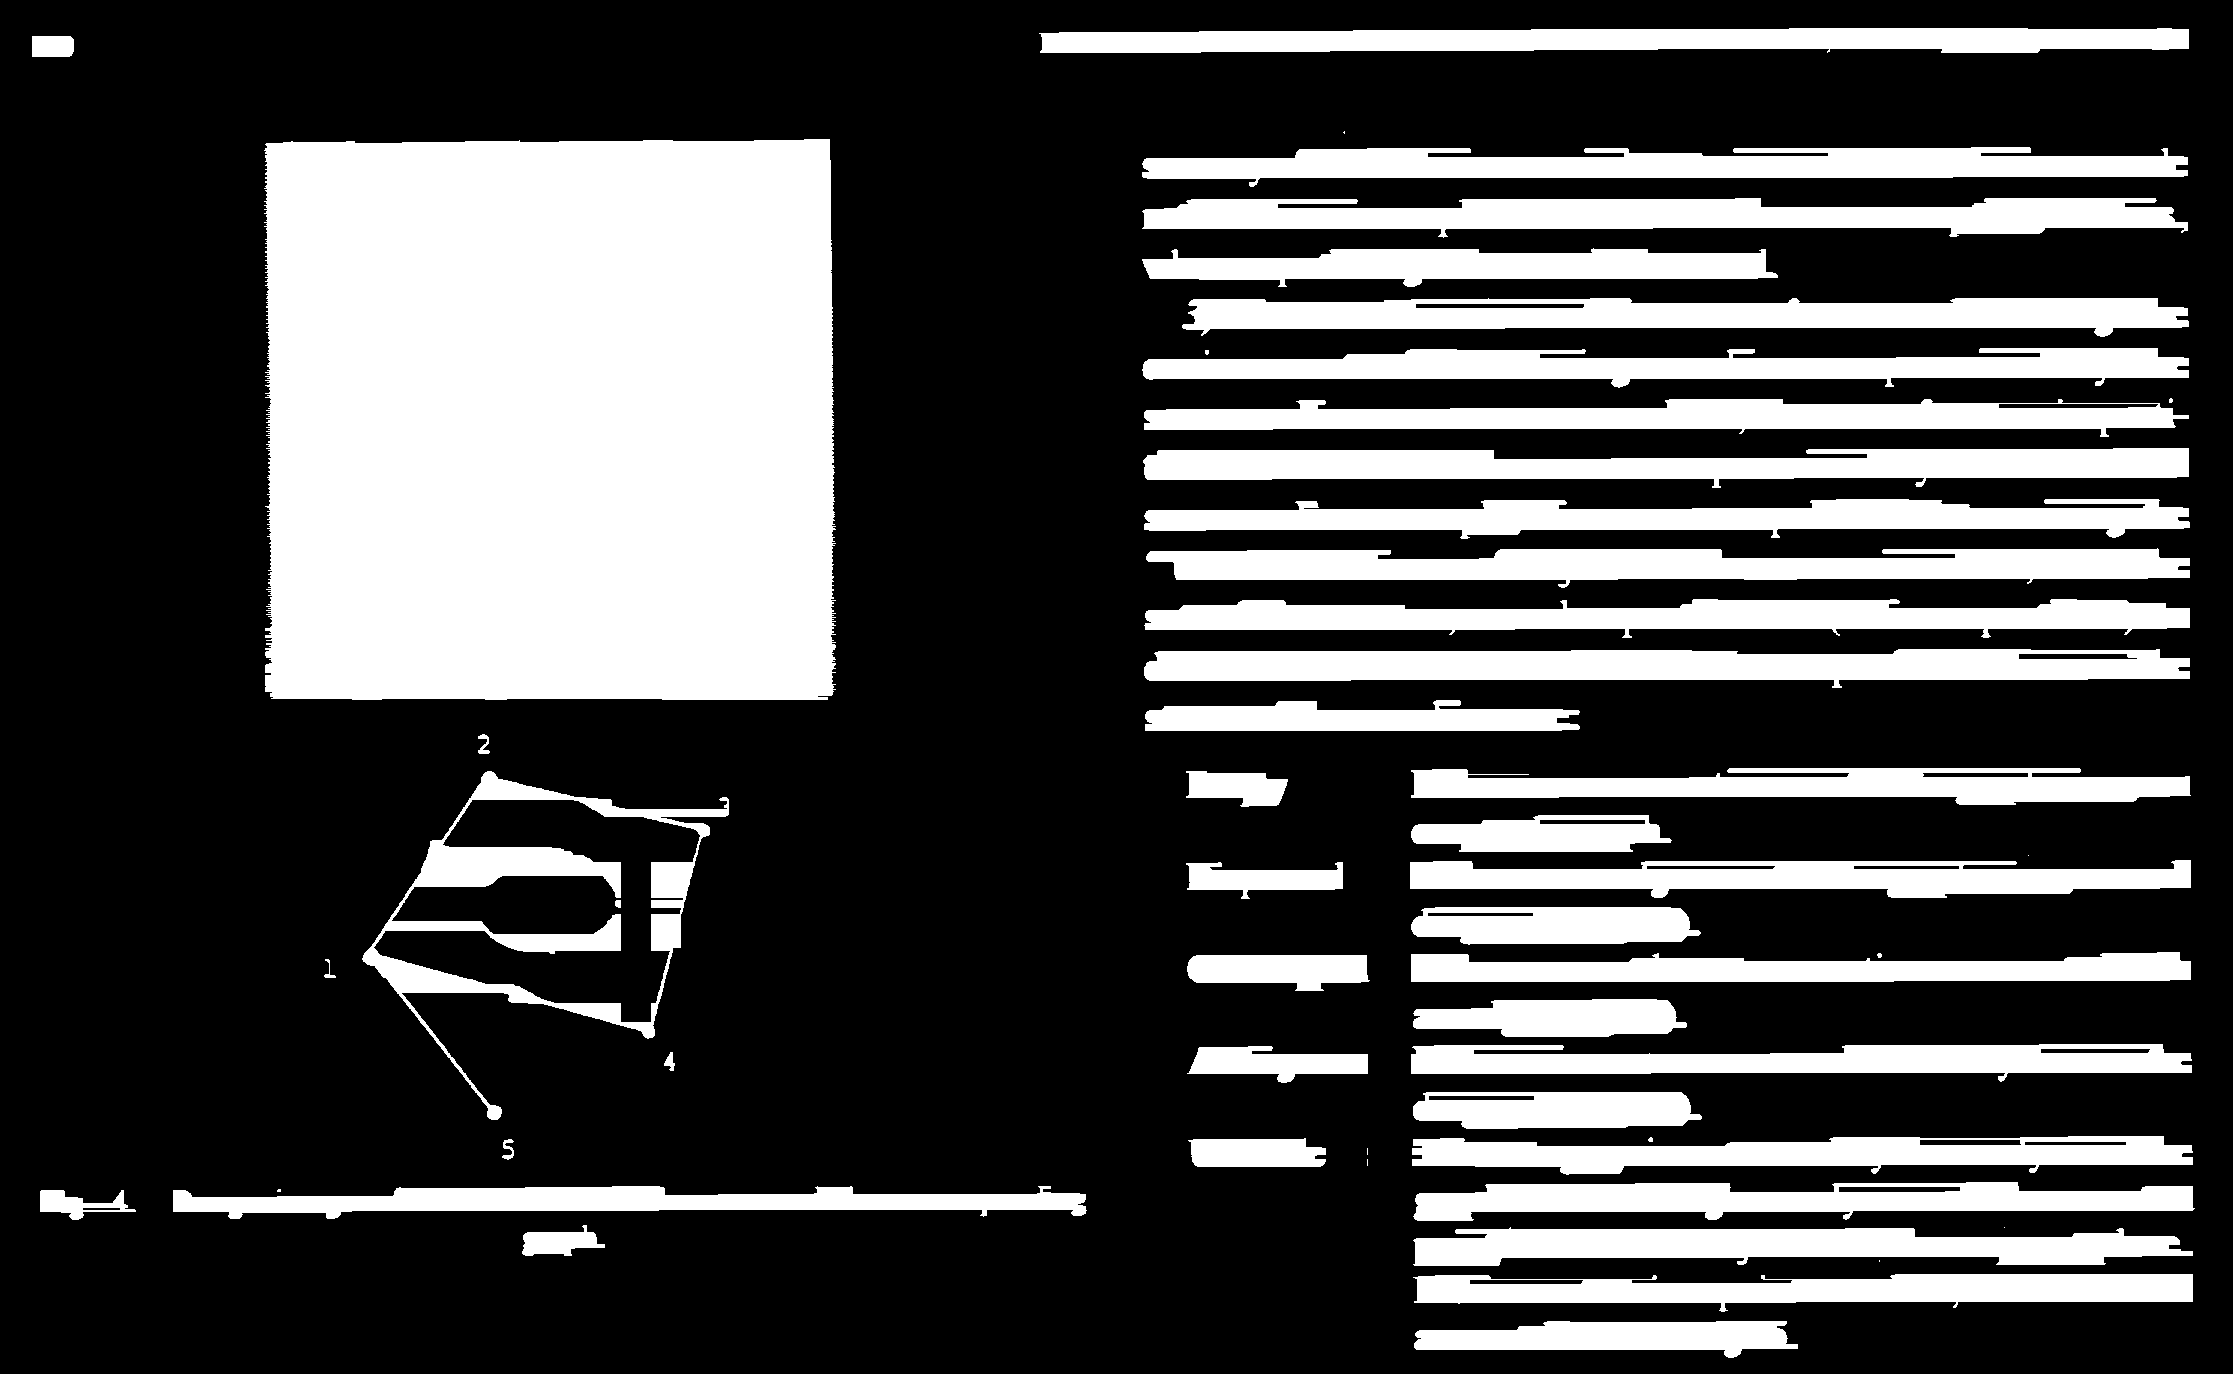
\includegraphics[height=4cm]{figures/step_6.png}
\caption{Passo (6)} \label{step_6}
\end{center}
\end{figure}

A Figura~\ref{step_6} apresenta o resultado da operação de fechamento da imagem da Figura~\ref{step_5} com um elemento estruturante de 1 \textit{pixel} de altura e 30 \textit{pixels} de largura. Como a operação de fechamento faz uma dilatação seguida de uma erosão, essa operação tem como objetivo ''fechar'' os buracos que possam existir nos componentes. Podemos observar que os componentes de uma mesma linha que estavam separados foram unidos, assim, no passo (7) é possível fazer uma boa identificação dos componentes conexos.

\begin{figure}[H]
\begin{center}
	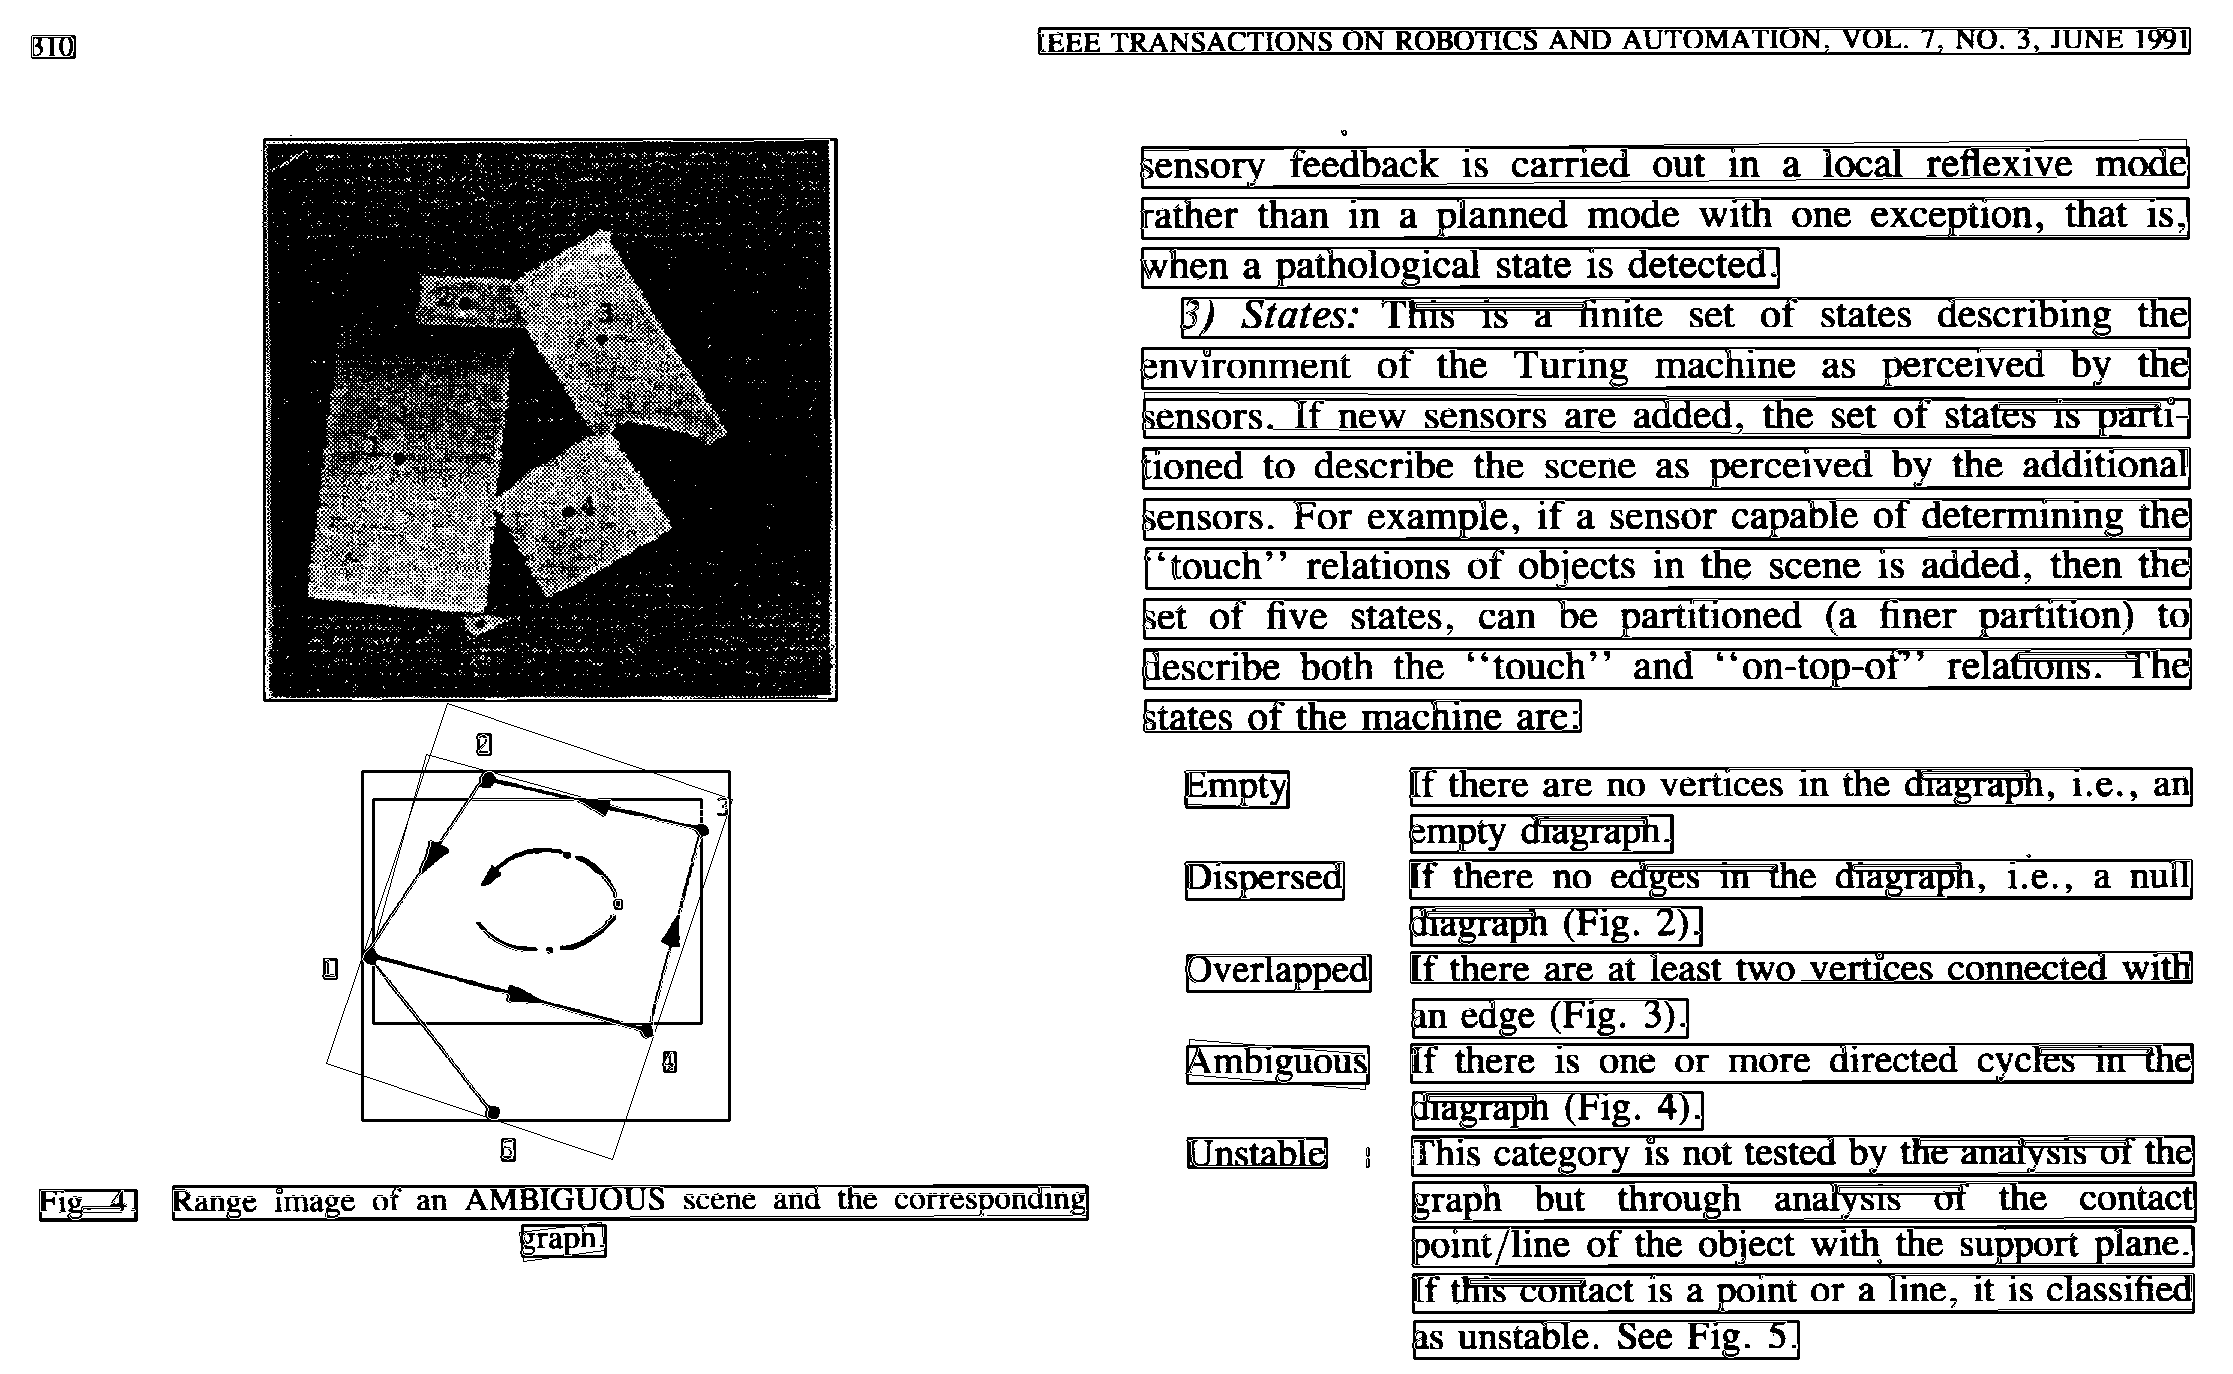
\includegraphics[height=4cm]{figures/step_7.png}
\caption{Passo (7)} \label{step_7}
\end{center}
\end{figure}

A Figura~\ref{step_7} apresenta o resultado da operação de detecção dos componentes conexos. Podemos observar que cada componente conexo existente na imagem da Figura~\ref{step_6} foi envolvido com um \textit{bounding box}. Para a identificação dos componentes conexos foi considerado a vizinhaça-4.

\begin{figure}[H]
\begin{center}
	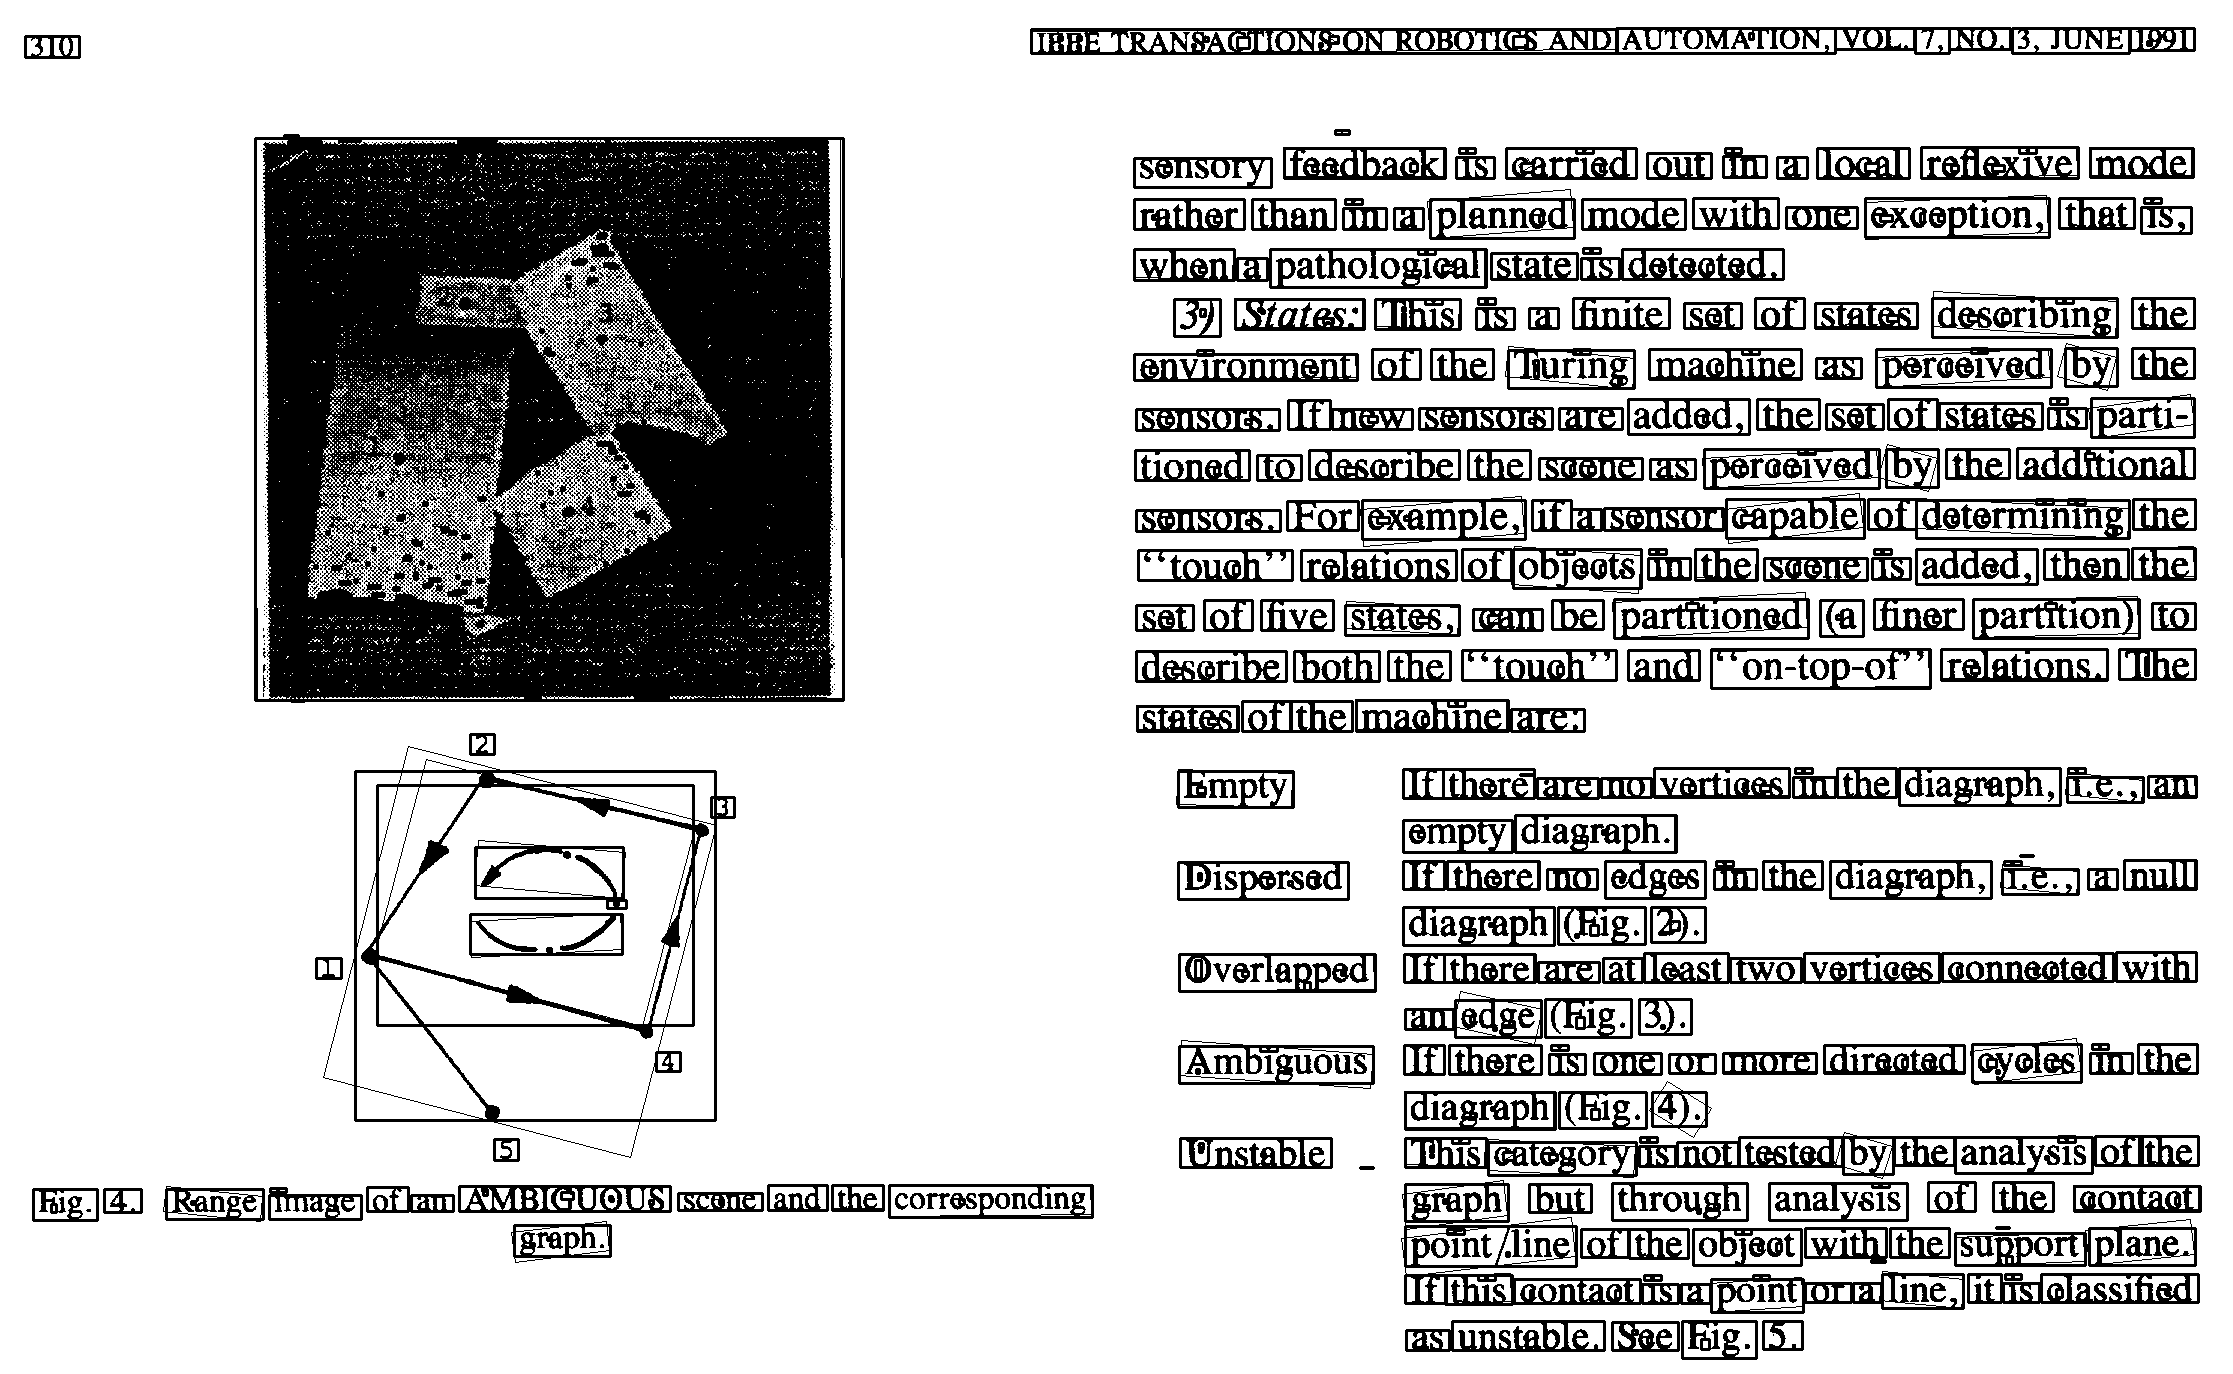
\includegraphics[height=4cm]{figures/step_10_1.png}
\caption{Passo (10.1)} \label{step_10_1}
\end{center}
\end{figure}

A Figura~\ref{step_10_1} apresenta o resultado da identificação dos componentes conexos e seus \textit{bounding boxex} correspondentes após a execução de 3 iterações da dilatação da imagem da Figura~\ref{bitmap_not} com um elemento estruturante de 1 \textit{pixel} de altura e 3 \textit{pixels} de largura.

\begin{figure}[H]
\begin{center}
	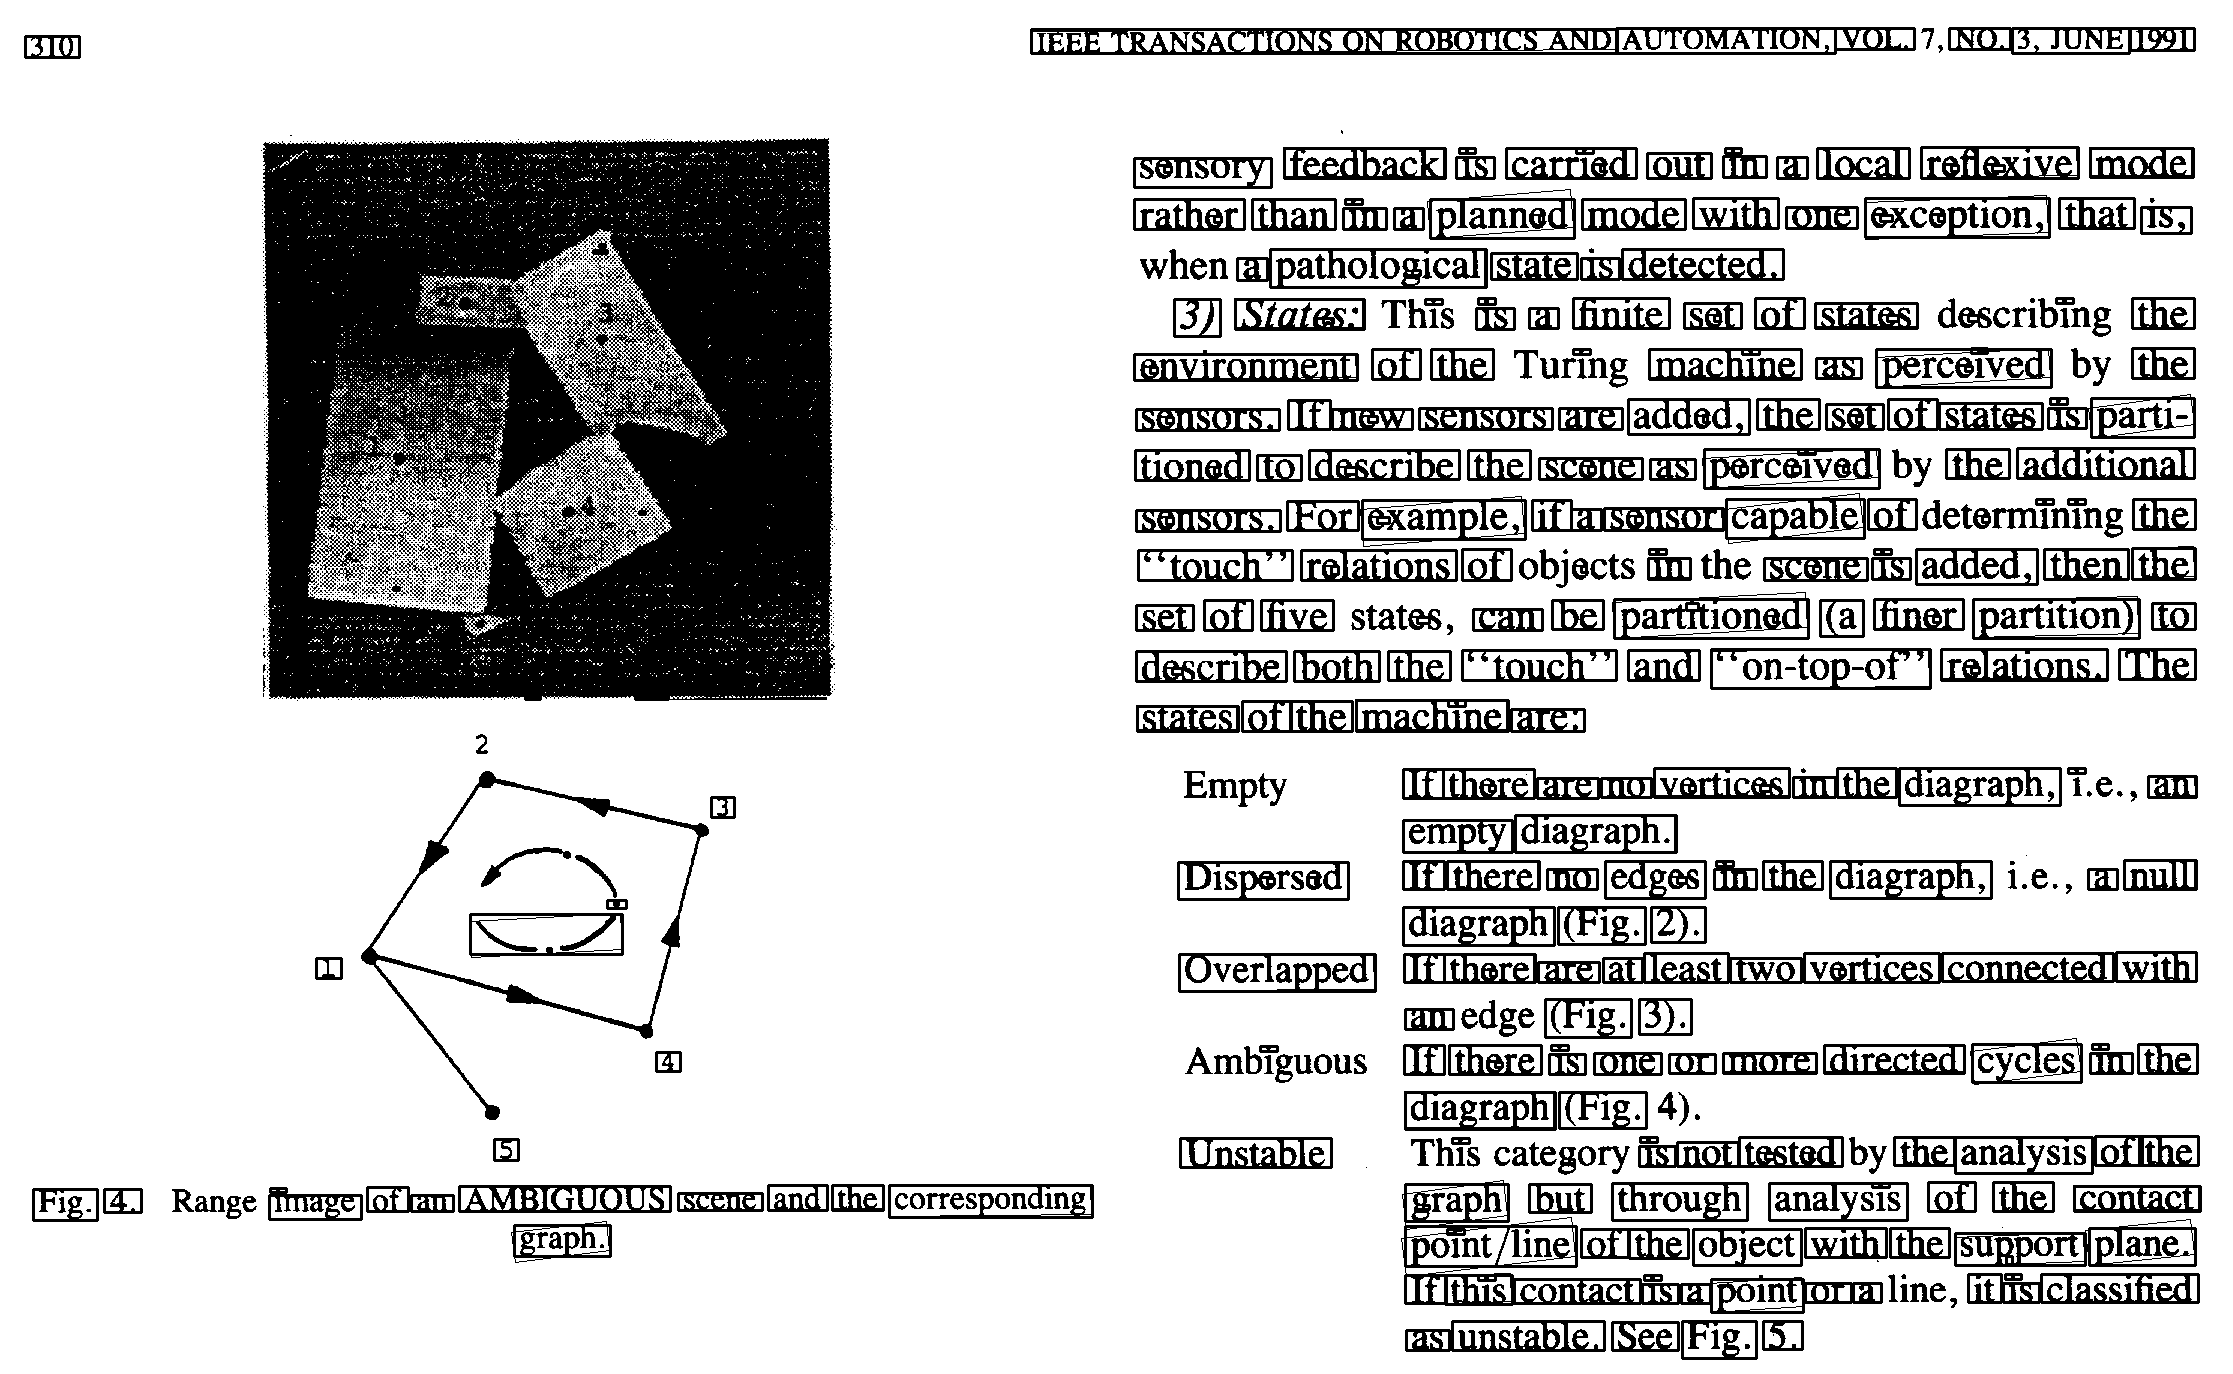
\includegraphics[height=4cm]{figures/step_10_2.png}
\caption{Passo (10.2)} \label{step_10_2}
\end{center}
\end{figure}

A Figura~\ref{step_10_2} apresenta o resultado da operação realizada na figura anterior, porém, só foram desenhados os \textit{bounding boxex} dos componentes que foram classificados como texto, de acordo com os resultados obtidos no passo (8.a) e (8.b) e a regra definida anteriormente. Assim, essa figura representa os componentes que foram reconhecidos como palavras.

A contagem do número de linhas e palavras foi realizada da seguinte forma: (i) a contagem de linhas foi realizada com base na imagem da Figura~\ref{step_7} e foram contabilizados somente os componentes que foram classificados como texto; (ii) a contagem de palavras foi realizada com base na imagem da Figura~\ref{step_10_2} e foram contabilizados todos \textit{bounding boxex} que foram classificados como texto.

Como resultado final temos que o número de linhas é 36 e o número de palavras é 305.

%------------------------------------------------

\section{Conclusão}

Podemos concluir que os resultados obtidos com as aplicações das técnicas de morfologia matemática para a detecção de linhas e palavras foram satisfatórios quanto a especificação do trabalho e que a criação de uma regra para classificação de texto e não texto com base nos cálculos do passo (8.a) e (8.b) se mostrou razoável para este objetivo, assim, consolida ainda mais os conceitos vistos em sala de aula.

%----------------------------------------------------------------------------------------
%	REFERENCE LIST
%----------------------------------------------------------------------------------------

\begin{thebibliography}{99} % Bibliography - this is intentionally simple in this template

\bibitem{b1} Welcome to opencv documentation! \href{https://docs.opencv.org/2.4/index.html}{https://docs.opencv.org/2.4/index.html} Acesso em: 04/05/2019.

\bibitem{b2} Pedrini, Hélio, and William Robson Schwartz. Análise de imagens digitais: princípios, algoritmos e aplicações. Thomson Learning, 2008.

\bibitem{b3} Matplotlib Version 3.0.3 \href{https://matplotlib.org/contents.html}{https://matplotlib.org/contents.html} Acesso em: 04/05/2019.
 
\end{thebibliography}

%----------------------------------------------------------------------------------------

\end{document}
